\chapter{Jets, Missing Energy, and Jet Response Templates}

Understanding the production and measurement of hadronic jets is 
of central importance to any hadron collider experiment.
Not only is pure multijet production the most common type of event,
but \textit{any} process can be accompanied by one or more jets
arising from initial- or final-state radiation of quarks and gluons.
Moreover, any mis-measurement of jet energies harms the experiment's 
ability to measure the imbalance in transverse energy, a key component
of many analyses. Understanding jet mis-measurement is thus highly important
for any analysis sensitive to this fake missing energy, such as the
one presented here.
Secs.~\ref{sec:cmsjet} and \ref{sec:cmsmet}
describe how jets and missing energy are measured at CMS, 
Sec.~\ref{sec:jetmismeas} summarizes the various sources of
jet mis-measurement, and Sec.~\ref{sec:jrt} details how
the jet response of the detector is actually measured
so that it can be accounted for.

\section{Jets at CMS}
\label{sec:cmsjet}
% brief theory of jet production
% ``multijet'' events most common at LHC

The production of jets, narrow cones of hadrons produced
in $pp$ collisions, was described in Sec.~\ref{sec:hadron_collider}.
Due to color confinement, isolated colored states cannot exist,
so high-energy quark and gluons that are expelled from the collision
point will \textit{hadronize} into a collection of hadrons in a 
cone around the initial momentum direction.

Jets consist predominantly of a mixture of charged an neutral 
hadrons, though they may also contain photons or leptons from
the decay of heavy-flavor hadrons. The charged hadrons
leave tracks in the tracker, and both the charged and neutral
hadrons deposit the majority of their energy in the HCAL.

\subsection{Jet clustering}
\label{sec:jetcluster}
A central task in event reconstruction is identifying individual
jets among the mess of tracks and energy deposits left
in the detector. To do this there exist various clustering algorithms
that attempt to reasonably group objects reconstructed by the detector
into separate jets.

As almost everything in a jet leaves
most of its energy in the calorimeters, 
one option is to just try to cluster the
calorimeter deposits into jets. However, calorimeters
have relatively low energy resolution, so CMS has developed
a ``particle-flow'' (PF) algorithm~\cite{CMS:pf} that combines calorimeter
information with that from the tracker and muon systems
to try to reconstruct each individual particle.
By using information from the higher-resolution tracker
and muon systems, a superior jet energy measurement is achieved.
A rough outline of the algorithm is as follows:
\begin{itemize}\setlength\itemsep{-1mm}
\item Match tracks in the tracker to tracks in the muon system.
These are PF muons.
\item Match remaining tracks to calorimeter deposits in the HCAL
and ECAL. These are PF charged hadrons (HCAL) or electrons (ECAL).
\item Any remaining calorimeter energy is assigned to 
PF neutral hadrons (HCAL) or photons (ECAL).
\end{itemize}

Once particles are identified, they are clustered into ``PF jets''.
There are a variety of ways to do this, but the most commonly used
at CMS and the one used for this analysis is the anti-$k_t$
algorithm~\cite{Cacciari:antikt}. Essentially, this defines a distance metric
parametrized by a characteristic size $R$ and iteratively combines objects
until a certain criterion is met. The parameter $R$ roughly corresponds
to the radius of the jet in $(\eta,\phi)$ space. For this analysis we use
a parameter of $R=0.4$. For analyses looking at boosted heavy objects
such as top quarks or Higgs bosons, resulting jets are often merged
into one large jet and a parameter of $R=0.8$ is commonly used.

\subsection{Pileup removal}
Blindly applying the above clustering procedures
over all particles in an event will lead to many particles from
pileup interactions being clustered into jets originating from
the primary vertex, artificially increasing their energies.
There are a number of ways to attempt to account for this.
The first, used for jets in this analysis, is known
as ``charged hadron subtraction'' (CHS). After the jets
are clustered, one simply removes all of the charged hadrons
whose tracks are unambiguously associated with a pileup vertex.
This method is simple, but does not account for any pileup contribution
from particles that aren't charged hadrons.

Another commonly used algorithm is called ``pileup per particle
identification'' (PUPPI). In this case, each particle is assigned a
weight based on the likelihood that it originates from pileup,
by considering the shape of the energy distribution in the immediate
vicinity of the particle. The particle energies are then scaled by this weight
when computing jet energies. The PUPPI algorithm gives slightly
better resolution in jet \pt and mass, and is used by analyses that
are sensitive to these quantities.

\subsection{Jet energy corrections}
The measurement of jet energies is imperfect, as there are
uncertainties from pileup contribution, calorimeter inefficiencies
and fluctuations, undetectable neutrinos, etc. 
CMS attempts to correct for this by calibrating the jet energy
scale as a function of various event and jet variables,
and correcting measured jet energies to give a more uniform response.
These corrections are together referred to as \textit{jet energy corrections},
or JECs.

The procedure is factorized into a number of discrete stages.
First, the L1 correction (unrelated to the L1 trigger) attempts to remove any residual 
energy coming from pileup interactions. The corrections
are derived from a MC sample of dijet events, processed
once with pileup interactions overlaid on the main event, 
and once with no pileup added. The quantity
$\pt^\mrm{PU}/\pt^\text{no PU}$ is fit in bins of jet $\eta$
as a function of mean event energy density $\rho$ (correlated
with the number of pileup interactions $N_\mrm{PU}$), jet
area $A$, and jet \pt.

Next, the L2 corrections account for imperfect and non-uniform
detector response. It is derived again on a MC sample of dijet
events, with L1 corrections already applied to the reconstructed
jet energies. The quantity $\pt^\mrm{reco}/\pt^\mrm{gen}$, where
$\pt^\mrm{reco}$ is the reconstructed jet energy and $\pt^\mrm{gen}$
is the generator-level jet energy (with neutrinos removed), is
fit in bins of jet $\eta$ as a function of jet $\pt$.

Finally, it is known that detector response is not modeled exactly
correctly in MC, so data-only L2 residual corrections are derived on 
a control sample of real data. \textit{Relative} corrections as a
function of jet $\eta$ are derived from a dijet sample, by comparing
the jet $\pt$ to a reference jet. \textit{Absolute} corrections, which
correct the $\eta$-independent absolute jet energy scale as a function
of \pt, are derived on a sample of \zjets or $\gamma$+jets events.

\subsection{b-jet tagging}
Many important processes contain final states with b quarks, including
the decays of top quarks, Higgs bosons, and SUSY particles. Identifying
the jets that originate from b quarks is a key method for reducing background.

Hadrons involving b quarks tend to be heavier and have longer lifetimes
than hadrons made from lighter quarks (for example, $B$ mesons haves masses
of $\sim$5\GeV and $c\tau$ values of $\mathcal{O}$(1 mm) when Lorentz-boosted). 
These properties can be used to
discriminate b jets from jets produced by light-flavor quarks or gluons.
Some variables/properties that provide discriminating power are:
\begin{itemize}\setlength\itemsep{-1mm}
\item Track impact parameters $d_z$ and $d_{xy}$. Charged hadrons from
b hadron decay tend to be slightly displaced from the primary vertex,
as the b hadron propagates a measurable amount before decaying.
Related to this is the impact parameter significance $\mrm{SIP}_{z,xy}$, found
by dividing the impact parameter by the uncertainty in its measurement.
\item Reconstructed secondary vertices. If there are enough high-quality
tracks from the decay of a displaced b hadron, a \textit{secondary vertex}
may be reconstructed which can indicate a b hadron was present in the jet.
\item Track \pt relative to the jet axis. Since b hadrons are heavy, their decay 
products tend to have more transverse momentum relative to the original
direction of propagation.
\item Presence of a charged lepton. Around 20\% of decays of b hadrons
result in an electron or muon, much higher than for non-b hadrons. Hence,
the presence of a charged lepton in a jet can indicate b decay.
\end{itemize}

These and other variables can be fed into a variety of multivariate algorithms
in order to identify b jets. A number of these algorithms have been designed and
tested by CMS~\cite{BTV_btagging}. For this analysis, we use the DeepCSV
algorithm~\cite{DeepCSV}, a deep neural network trained on track-level variables
to discriminate between b, c, bb, cc, and light-flavor jets.

Three nominal working points are set for the trained algorithm, corresponding 
to light-flavor fake rates of roughly 0.1\%, 1\%, and 10\%. We use the medium working point,
which achieves an efficiency of 68\% and fake rates of 12\% and 1.1\% for c and light-flavor
jets, respectively, for jets with $\pt>20\GeV$.


\section{Missing transverse energy at CMS}
\label{sec:cmsmet}

As protons are composite particles, the underlying collisions at the LHC are between
partons carrying an undetermined fraction of the total momentum. Hence, the lab frame is
in general not the center-of-mass frame, and the total momentum of the colliding system
is boosted along the beam direction. The \textit{transverse} momentum, orthogonal
to the beamline, on the contrary should be zero (technically, the partons can have a
transverse momentum on the scale of the proton mass of a few hundred\MeV, but this
is negligible at the LHC energy scales).

If all produced particles were perfectly measured, then, the vector sum of their \vpt
values should be zero. This is not the case in practice, however. Any measured imbalance in
the transverse momentum is referred to as \textit{missing transverse momentum/energy}, referred
to variously as $\vMet$, $\vec{E}_\mrm{T}^\mrm{miss}$, $\vec{\slashed{E}}_\mrm{T}$, or MET.
Real \ptmiss comes from undetectable particles such as neutrinos or hypothetical LSPs.
Fake \ptmiss can arise from effects like pileup contamination or imperfect detector
response; a central part of this analysis will be measuring the CMS jet response distributions
to estimate contribution from events with fake \ptmiss from mis-measured jets.

At CMS, the primary way of computing \ptmiss, called PF-MET, is to simply sum the momenta
of all reconstructed particle-flow candidates. The raw \ptmiss can thus be defined
\be
\vec{\slashed{E}}_\mrm{T}^\mrm{raw} = -\sum_{i\in\mrm{PFcands}} \vec{p}_{\mrm{T},i}.
\ee

However, we know that detector response is imperfect, and we have already calibrated for
this when deriving jet energy corrections. So the \ptmiss measurement is easily improved
by simply applying the same jet energy corrections to the jets before computing \ptmiss.
We can re-write thaw raw \ptmiss as
\be
\vec{\slashed{E}}_\mrm{T}^\mrm{raw} = -\sum_{i\in\mrm{jets}} \vSS{p}{\mrm{T},i}{\mrm{raw}}
- \sum_{i\in\mrm{uncl}} \vec{p}_{\mrm{T},i},
\ee
where the first sum is over all jets and the second is over any
particle-flow candidates not clustered into jets.
Then the JEC-corrected, or type 1-corrected, \ptmiss can be computed by
simply replacing the jet momenta with their corrected values:
\be\begin{split}
\vec{\slashed{E}}_\mrm{T}^\text{type-1} &= -\sum_{i\in\mrm{jets}} \vSS{p}{\mrm{T},i}{\mrm{corr}}
- \sum_{i\in\mrm{uncl}} \vec{p}_{\mrm{T},i} \\
&= \vec{\slashed{E}}_\mrm{T}^\mrm{raw} - \sum_{i\in\mrm{jets}}\left(\vSS{p}{\mrm{T},i}{\mrm{corr}}-\vSS{p}{\mrm{T},i}{\mrm{raw}}\right).
\end{split}\ee

This type 1-corrected \ptmiss is the version used in this analysis.

% missing energy
% contribution from mis-measured jets
% T1 corrections

\section{Sources of jet mis-measurement}
\label{sec:jetmismeas}
For the purposes of estimating background from QCD multijet events (Chapter~\ref{chap:qcd}),
we will be interested in modeling the ``response'' of the CMS detector to jets.
That is, for a jet with a true \pt of $p_\mrm{T}^\mrm{true}$, what will be the
measured $p_\mrm{T}^\mrm{reco}$? Jet measurement is an inherently random process, so the response
will be given in the form of a probability density function in the variable
$p_\mrm{T}^\mrm{reco}/p_\mrm{T}^\mrm{true}$. 

Looking ahead, Fig.~\ref{fig:jrt_examples} shows a 
few examples of these functions measured in simulation (called jet response templates, or JRTs).
It is found that the templates are described well by a central Gaussian core (red),
with larger, non-Gaussian tails (green).
Details on the exact derivation of these functions, and the procedure for fitting
the core and tails, are given in Sec.~\ref{sec:jrt}. For now, it is sufficient
to know that they are measured in simulation by matching reconstructed jets
(``reco jets'') to generator-level jets (``gen jets'') and comparing their \pt values.

The size and shape of the core are due to standard stochastic smearing in the calorimeters. 
The width of this Gaussian core, referred to
as the ``jet resolution'', generally falls as $1/\sqrt{E}$. This is illustrated in 
Fig.~\ref{fig:jrt_res_pt} (left), which shows the measured
resolution improving as jet \pt increases.

The tails, on the other hand, come from rarer events in which the measured jet \pt 
is much further from the true value. These types of events
are harder to model, but as we will see are critically important for the 
QCD estimate method to work. In order for a multijet event to populate the high-\ptmiss signal regions, 
generally one or more jets must be badly mis-measured
(i.e., reside in the tails of the response functions).

The sources of the measured tails fall into two categories. The first, ``real sources'', 
are due to real effects that are present in the data we are interested in modeling. 
The second, ``fake sources'', are due to features of the simulation or template-derivation 
methodology that are not reflected in the actual data. 
We seek to model the first category as accurately as possible, 
and remove events from the second category so that
they do not artificially enhance the tails of the templates.
\begin{itemize}
\item{Real sources}
   \begin{itemize}
   \item Neutrinos from heavy-flavor decay (mostly in jets from b quarks). This enhances the \emph{left} tails, and is the
   reason for deriving separate templates for b jets (see Fig.~\ref{fig:jrt_res_pt} (right)).
   \item Reconstruction errors, e.g. a badly reconstructed high-\pt track that greatly increases the reconstructed jet \pt. This generally enhances the \emph{right} tails.
   \item Holes or cracks in the detector that cause part of the reconstructed jet to go ``missing''. This enhances the \emph{left} tails.
   \item Overlap with a pileup jet. This enhances the \emph{right} tails.
   \end{itemize}
\item{Fake sources}
   \begin{itemize}
   \item Gen or reco jet ``splitting''. i.e. for a single gen (reco) jet, the corresponding reco (gen) jet is clustered as two different jets, and only one gets matched. 
   Depending on the direction, this enhances \emph{both} tails.
   \item Mis-matching a gen jet to a reconstructed pileup jet. This generally enhances the \emph{left} tails.
   \item Holes in the simulated calorimeter that are not present in the real data. This enhances the \emph{left} tails.
   \end{itemize}
\end{itemize}


\section{Derivation of jet response templates}
\label{sec:jrt}

The jet response templates are measured in simulation, by matching gen and reco jets
using the distance measure $\Delta R = \sqrt{\Delta\phi^2+\Delta\eta^2}$.
Section~\ref{sec:jrt_matching} describes the gen/reco jet matching procedure, 
and measures taken to prevent fake matches that artificially enhance the tails of the templates.
Section~\ref{sec:jrt_fits} describes the methodology for fitting the core/tails of the
derived templates, and the procedure to correct the template resolutions for known
differences in jet resolution between data and MC.

\begin{figure}[htbp]
  \begin{center}
    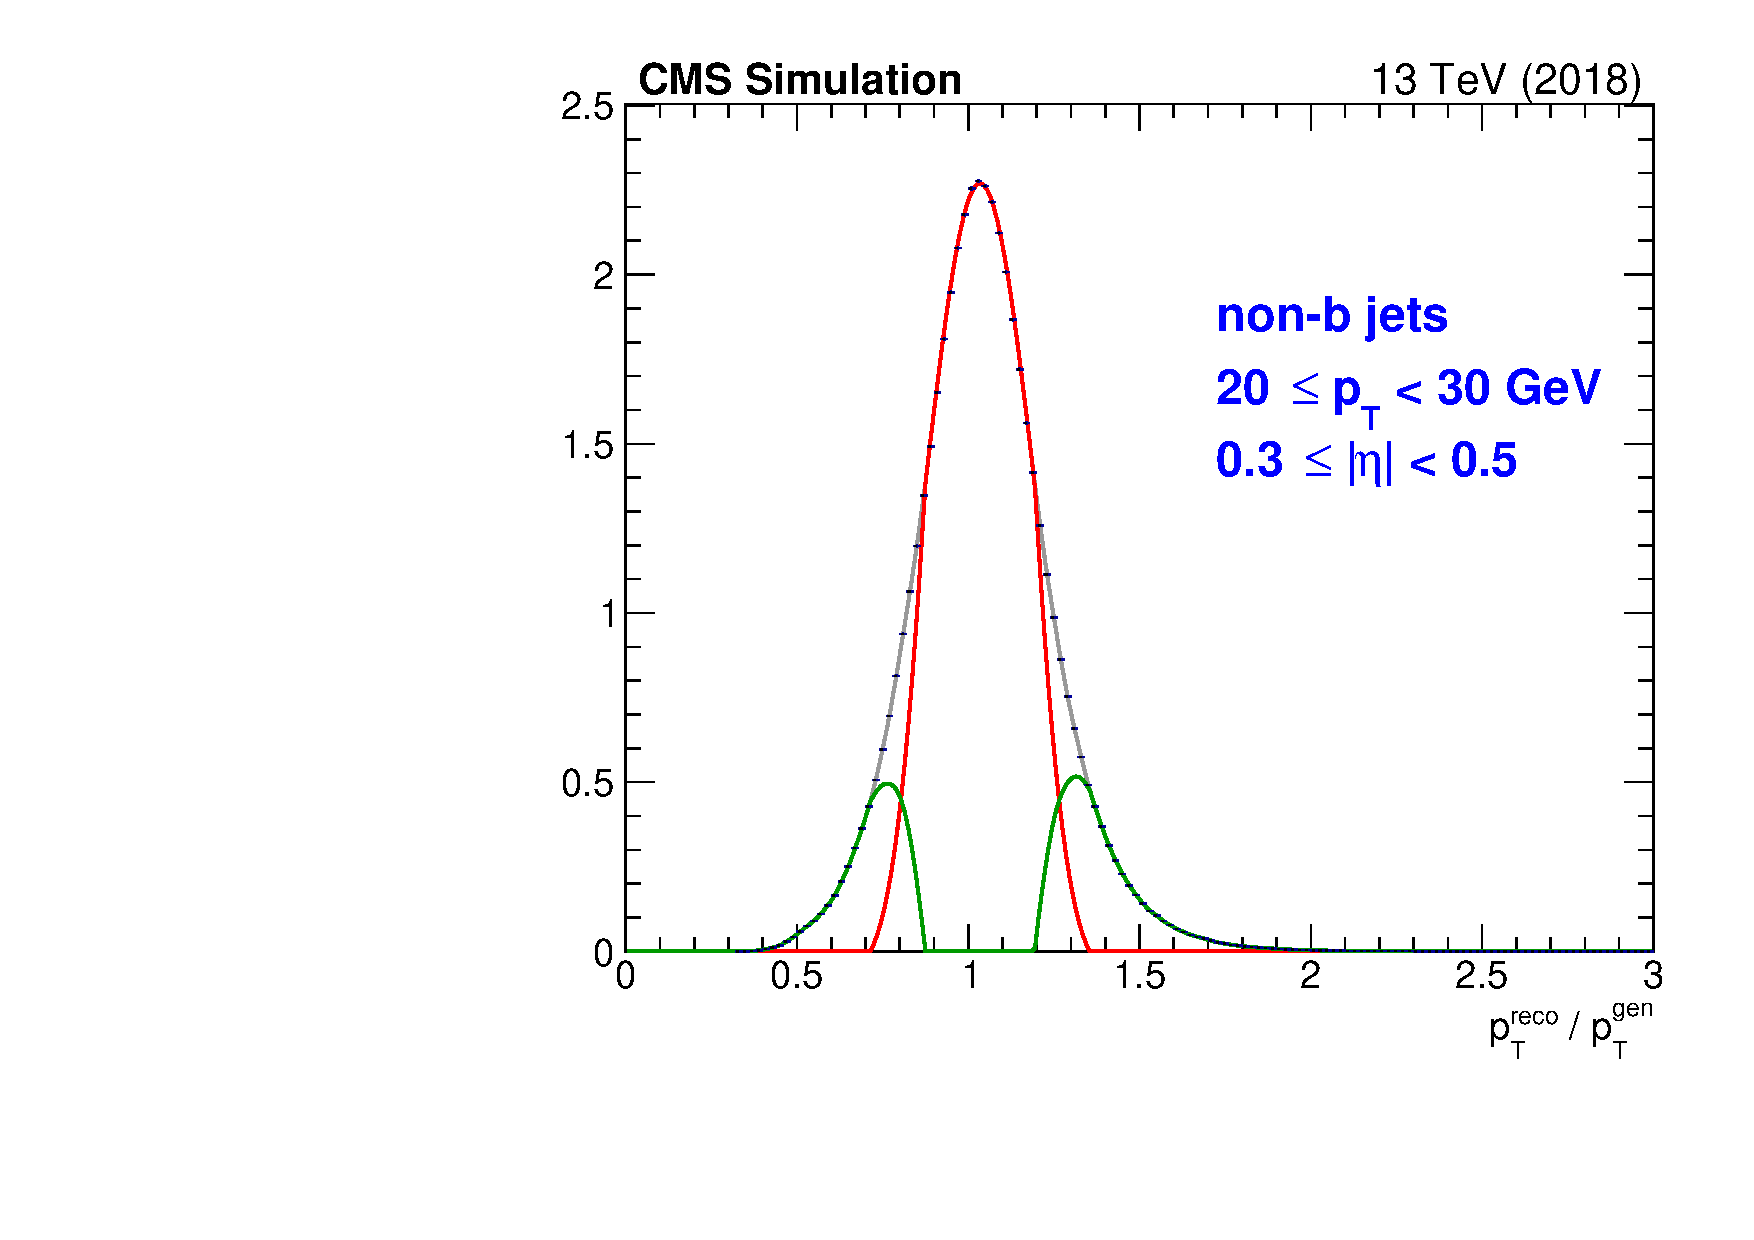
\includegraphics[width=0.45\textwidth]{figs/jetmet/pt01_eta01_nonbjets_lin.pdf}
    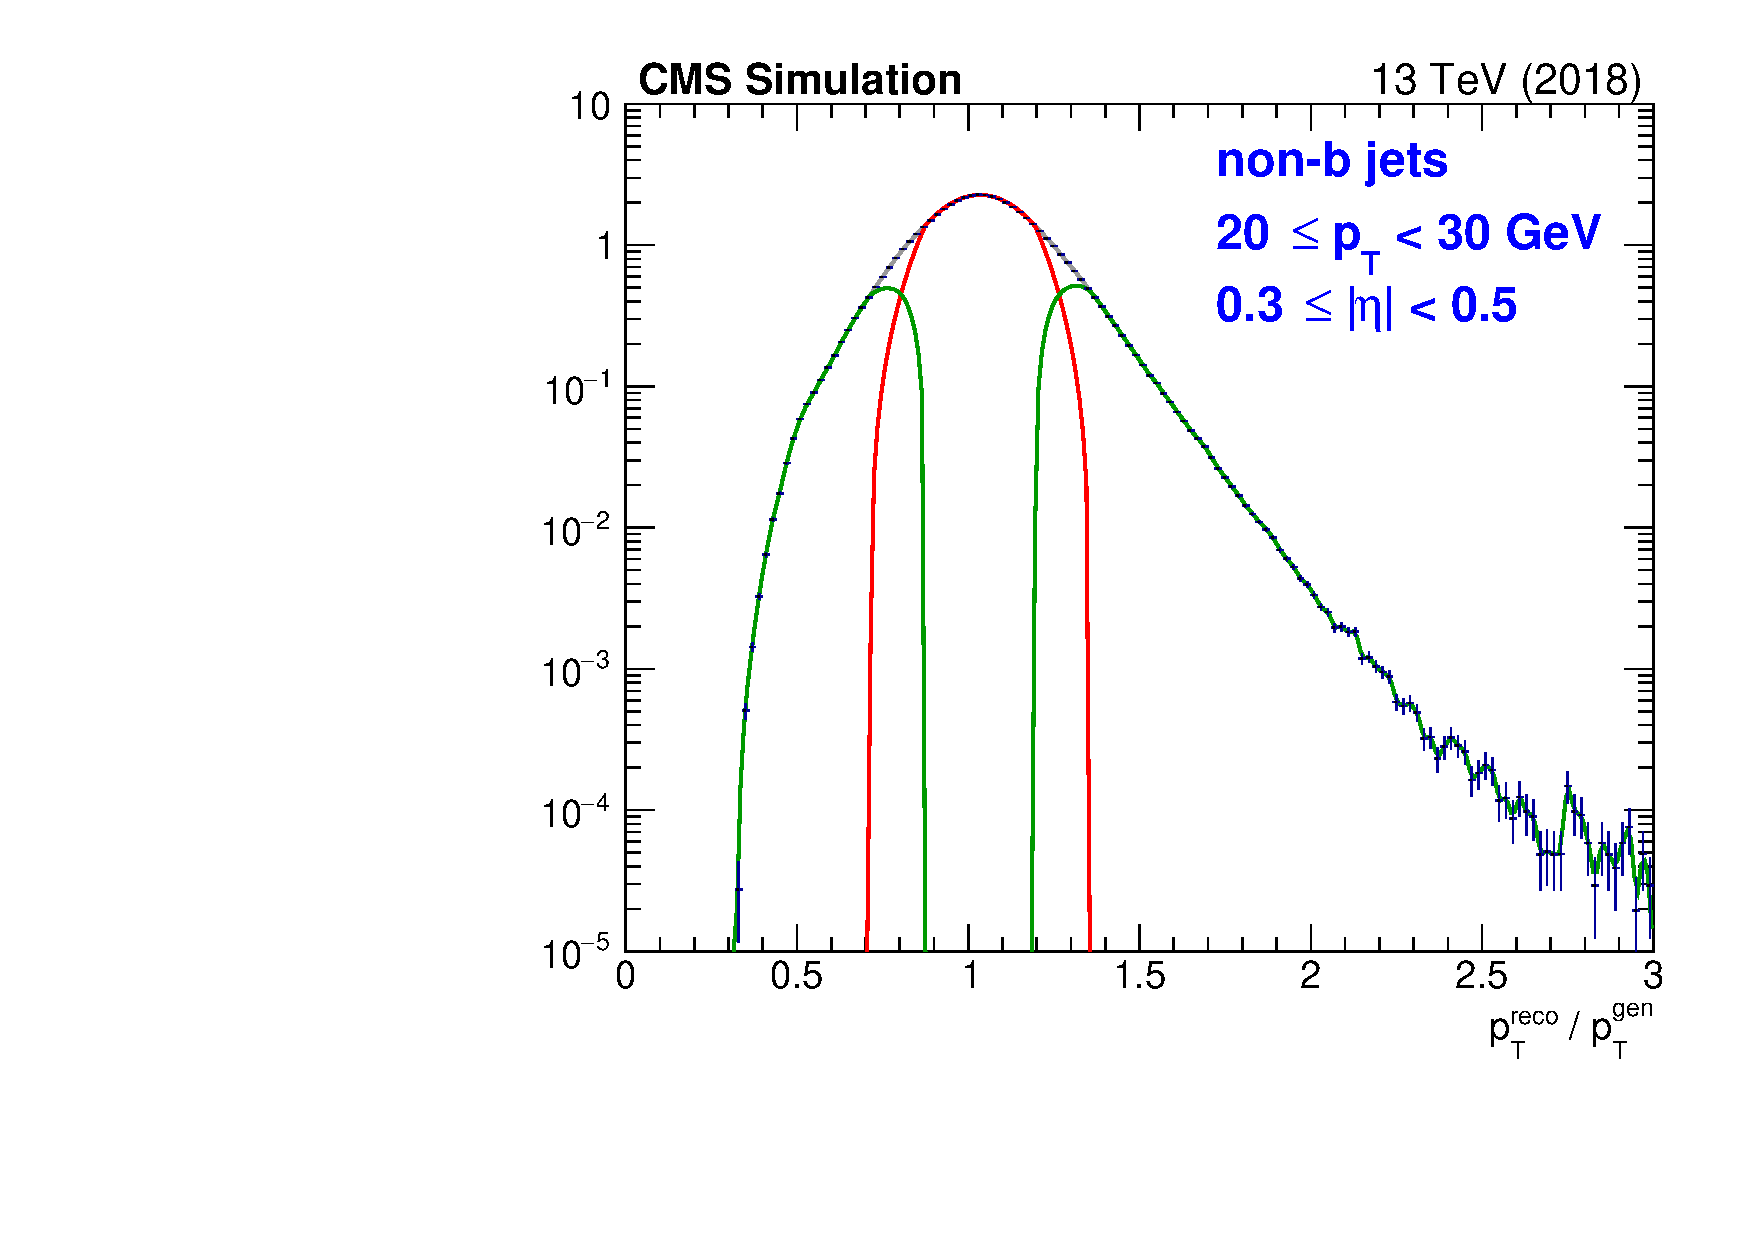
\includegraphics[width=0.45\textwidth]{figs/jetmet/pt01_eta01_nonbjets_log.pdf} \\
    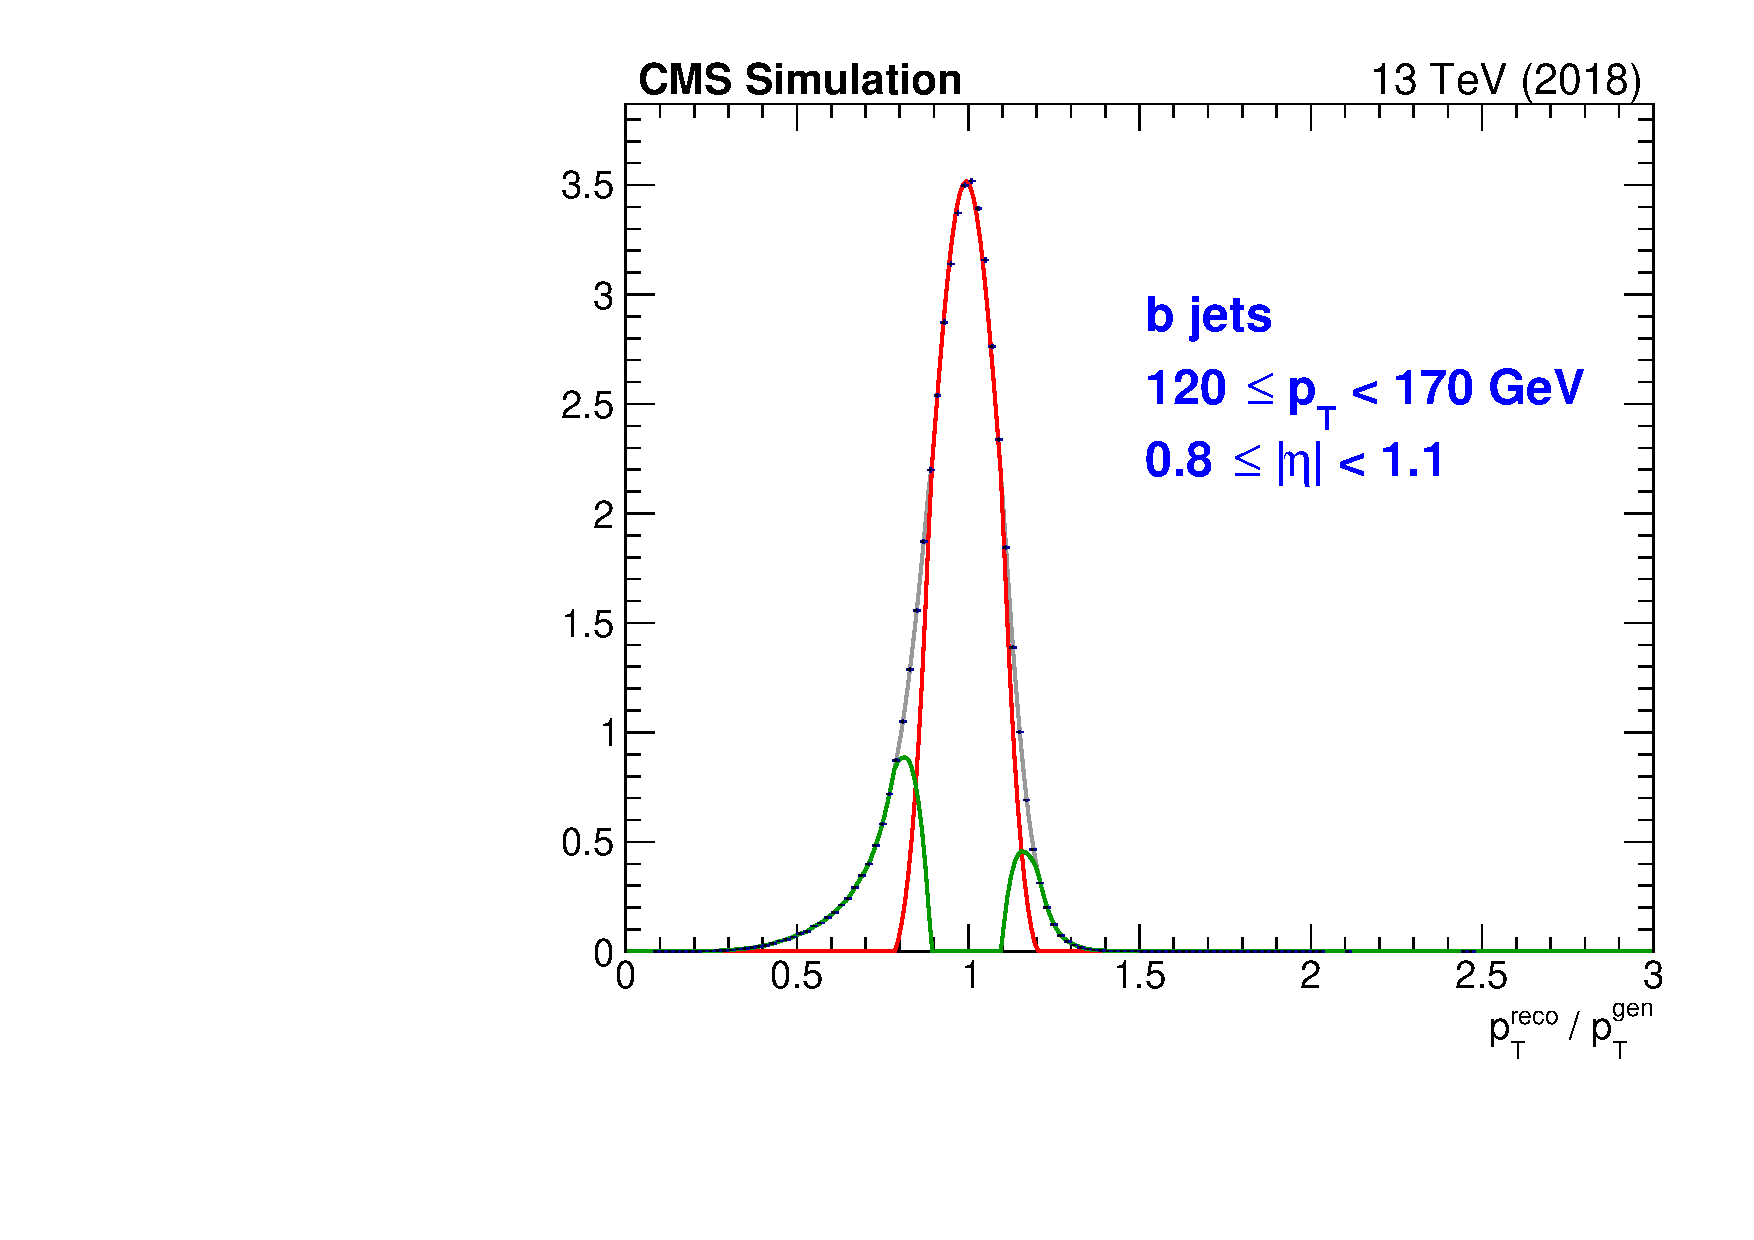
\includegraphics[width=0.45\textwidth]{figs/jetmet/pt05_eta03_bjets_lin.pdf}
    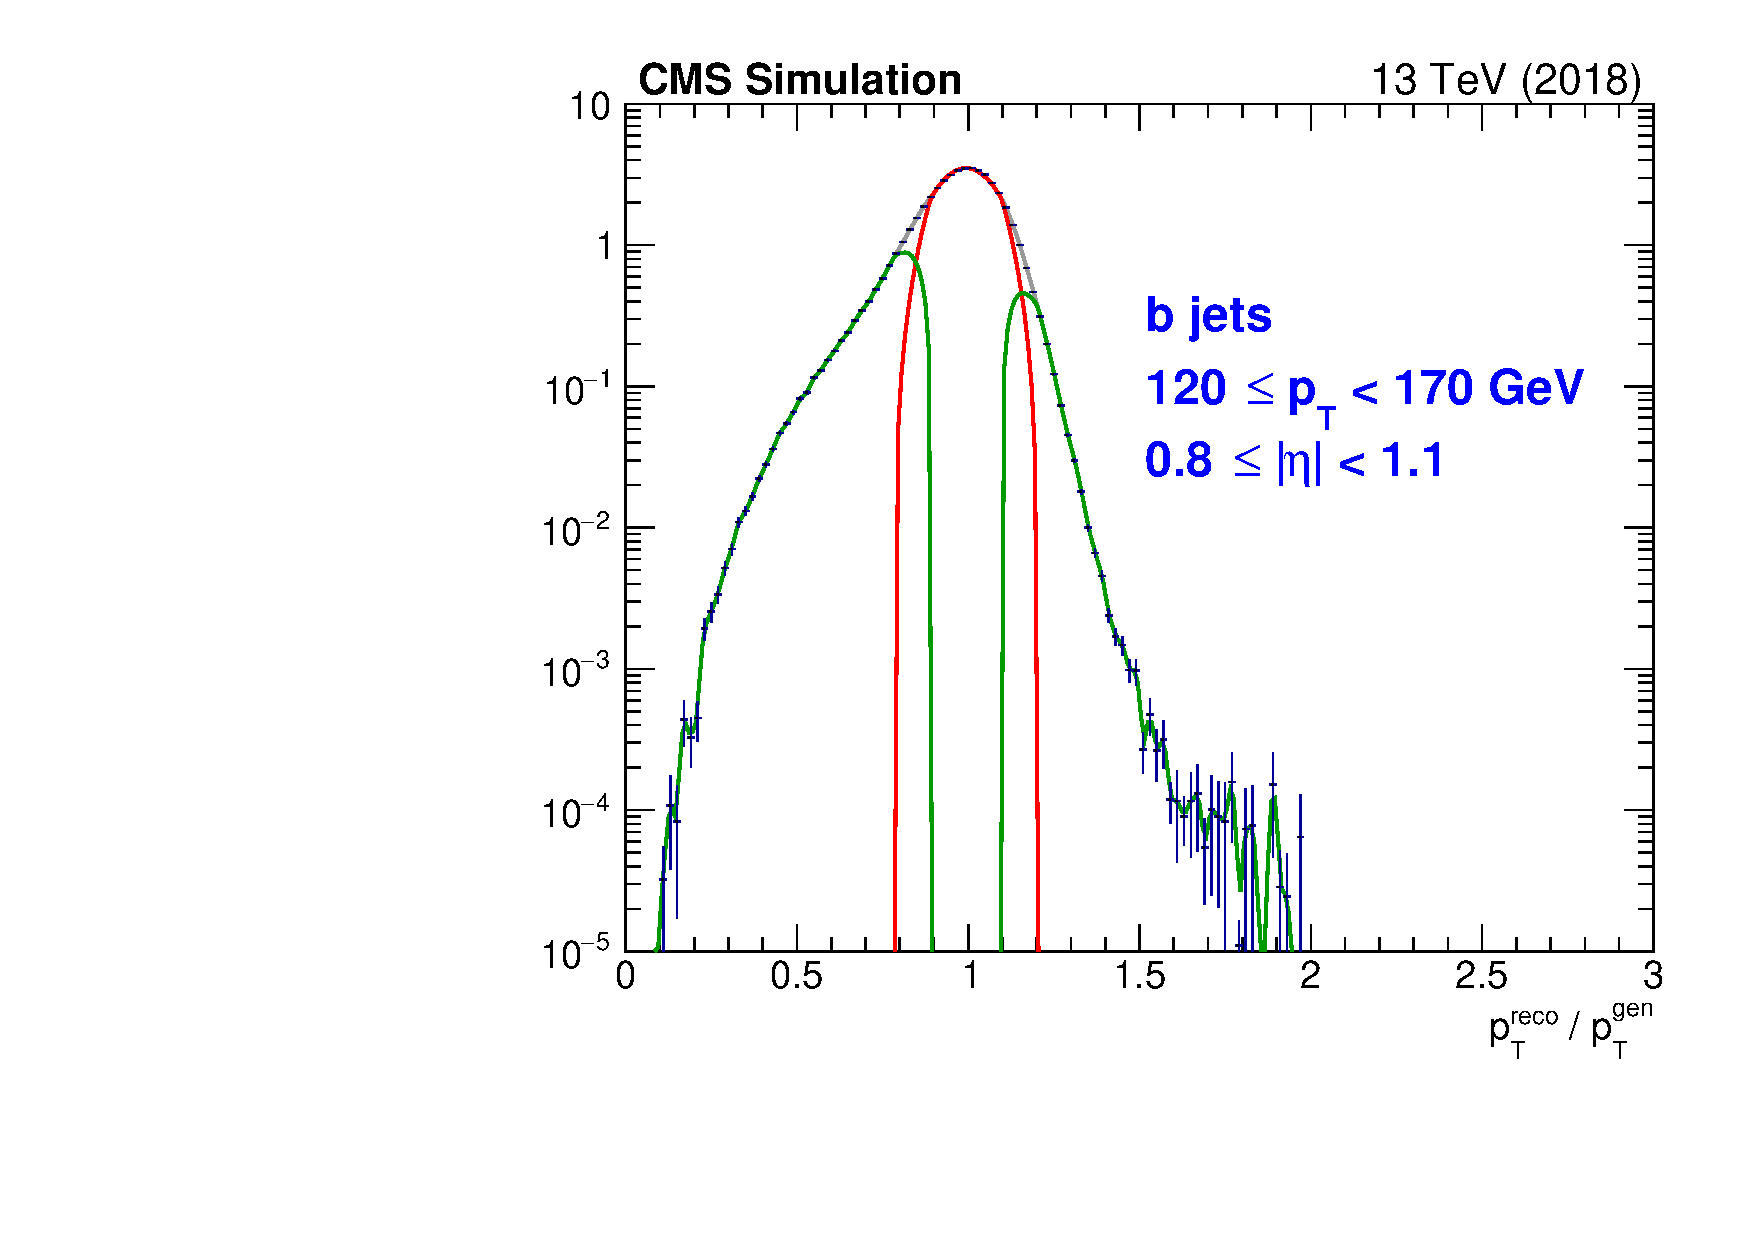
\includegraphics[width=0.45\textwidth]{figs/jetmet/pt05_eta03_bjets_log.pdf} \\
    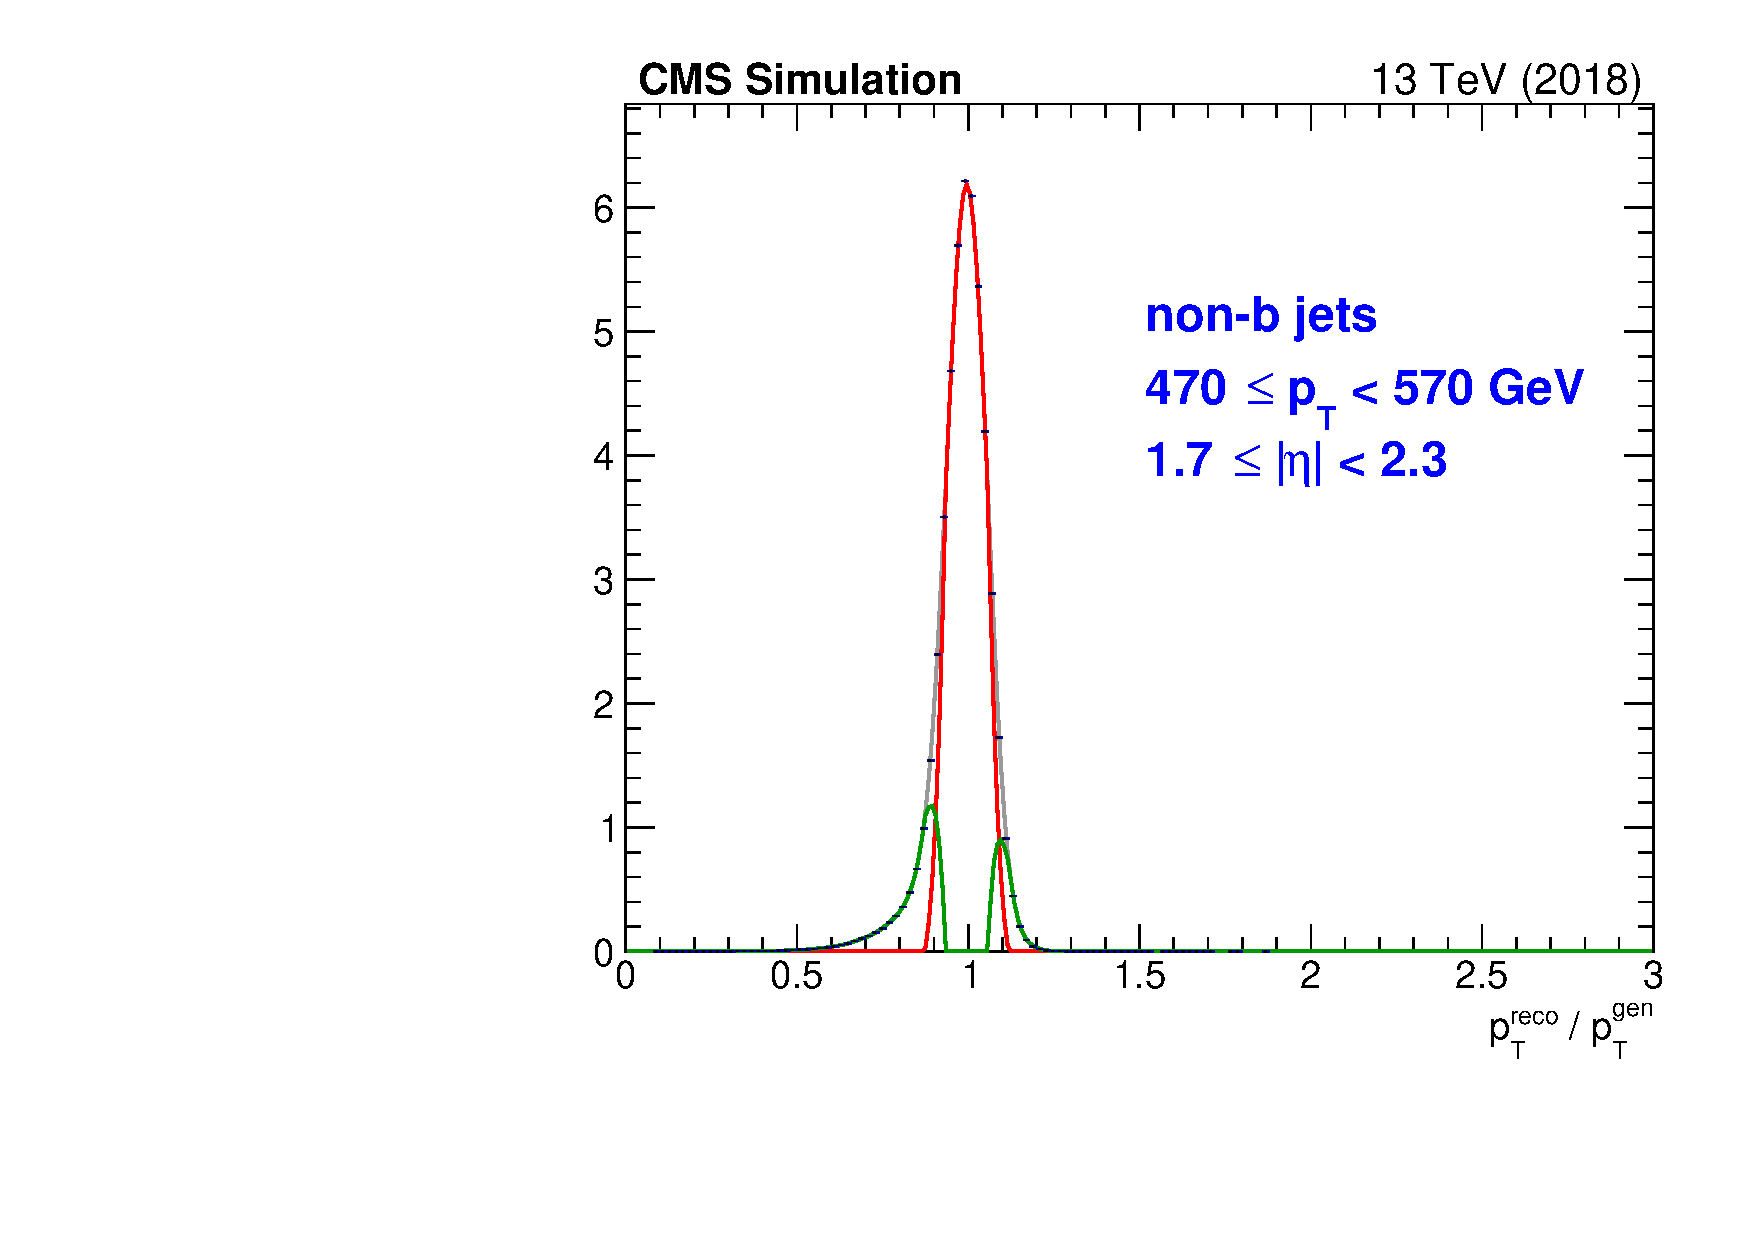
\includegraphics[width=0.45\textwidth]{figs/jetmet/pt10_eta06_nonbjets_lin.pdf}
    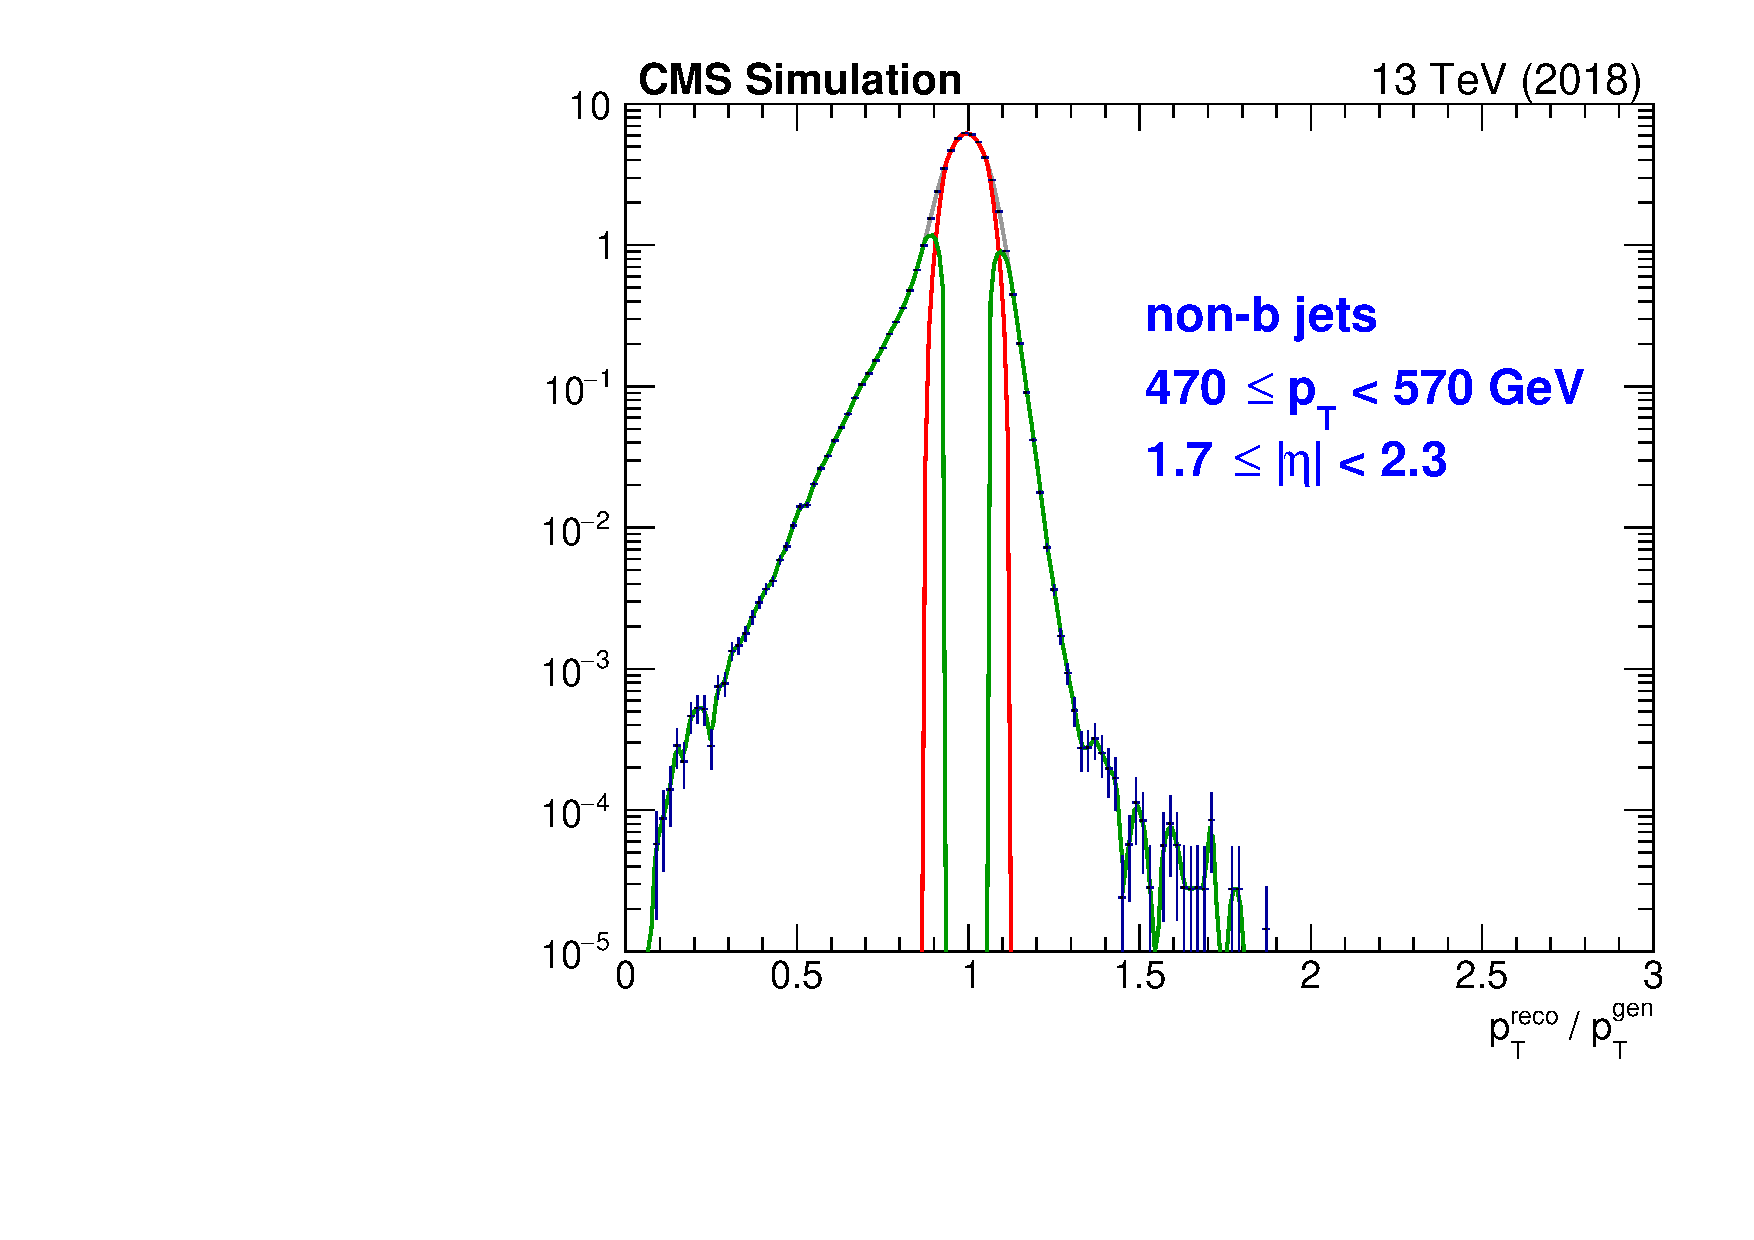
\includegraphics[width=0.45\textwidth]{figs/jetmet/pt10_eta06_nonbjets_log.pdf} \\
    \caption{A selection of three example jet response templates for various \pt/$\eta$/b-jet bins, shown in linear (left) and log (right) scales.
    The dark blue points are the raw templates. The red curves are the fitted Gaussian ``cores'' of the templates, and the green
    curves are the ``tails'', as described in Section~\ref{sec:jrt_fits}.
           }
    \label{fig:jrt_examples}
  \end{center}
\end{figure}

\begin{figure}[ht]
  \begin{center}
    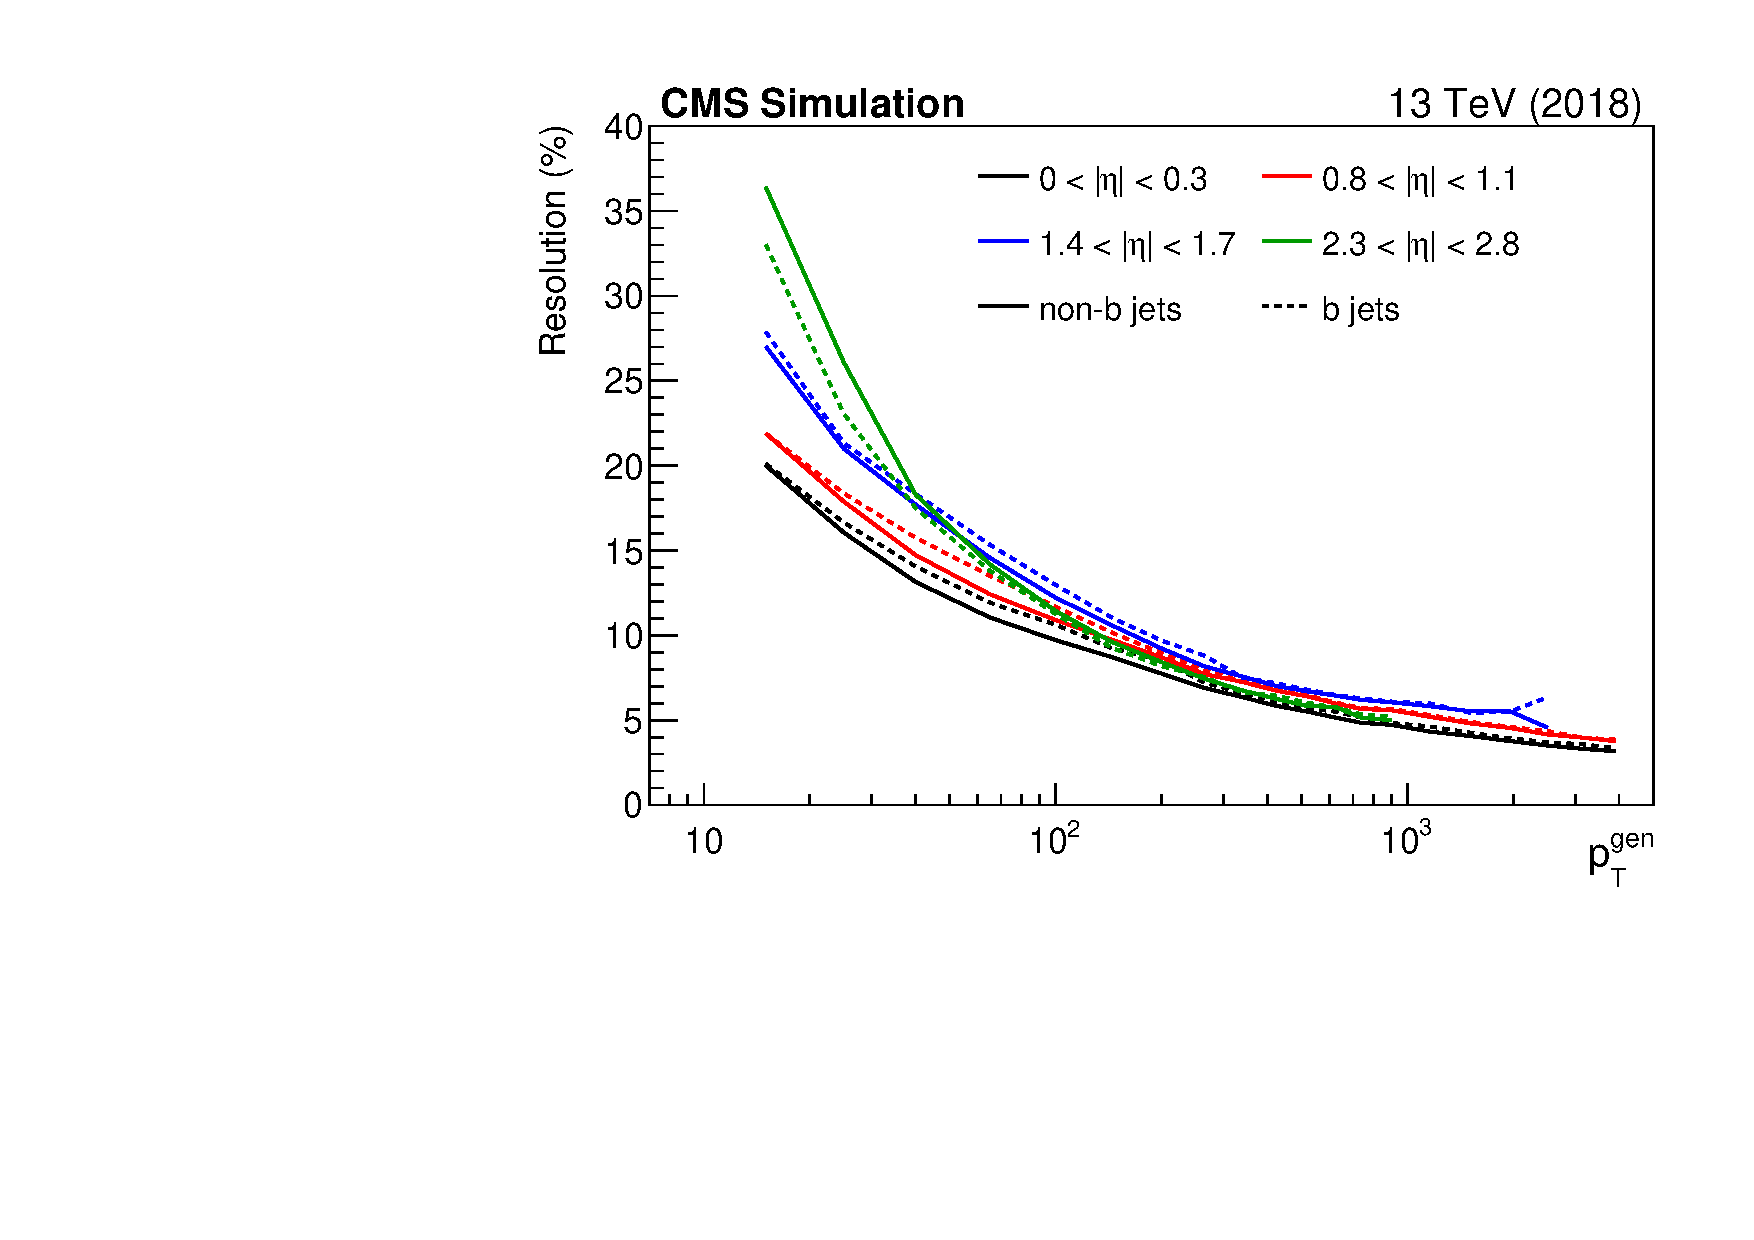
\includegraphics[width=0.49\textwidth]{figs/jetmet/resolution_vs_pt.pdf}
    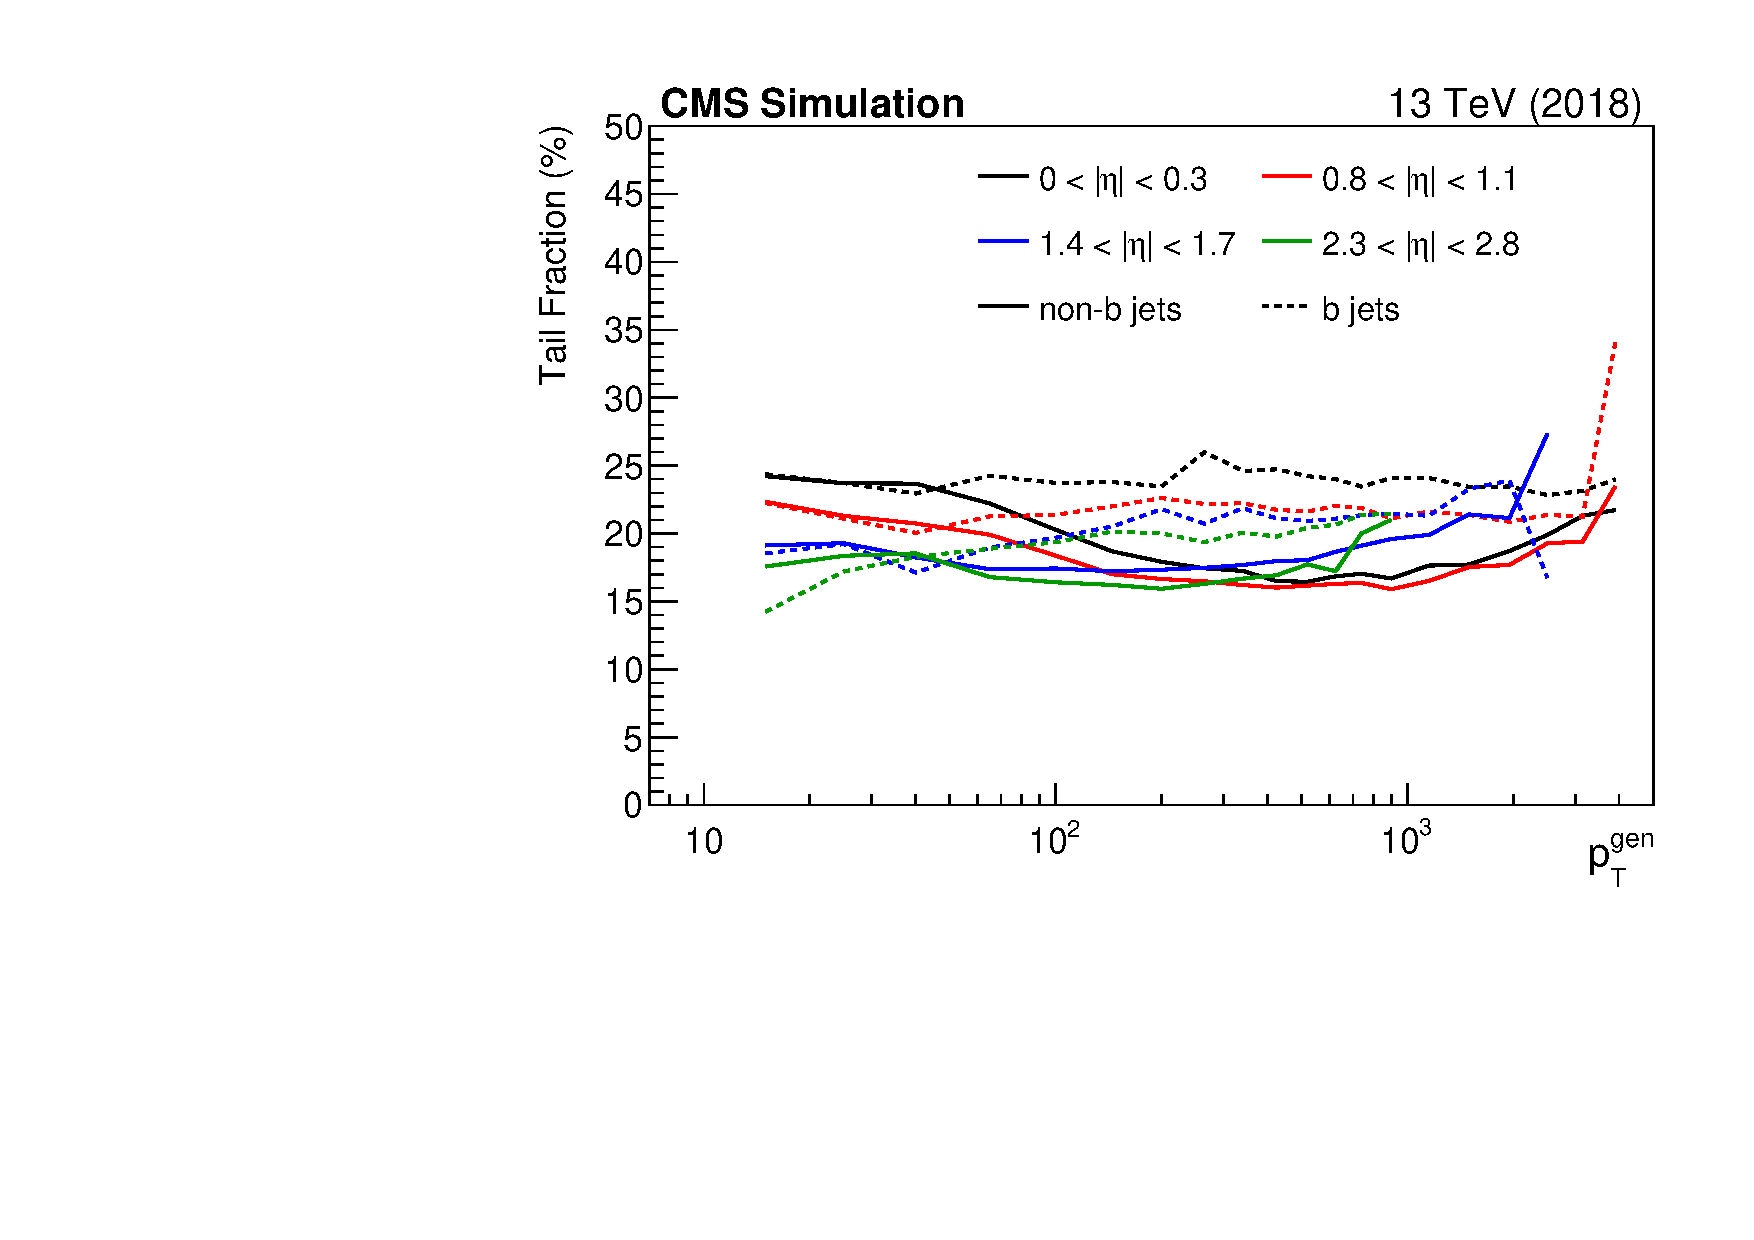
\includegraphics[width=0.49\textwidth]{figs/jetmet/tailfrac_vs_pt.pdf}
    \caption{(left) Jet energy resolution (defined as the width of the fitted Gaussian core) as a function of generator-level jet \pt, as measured in 2018 MC. 
    Resolution improves as jet \pt increases, and generally degrades as $\eta$ increases.
    (right) The fraction of the jet response function that resides in the fitted tails (as opposed to the Gaussian core) as a function of generator-level jet \pt, 
    as measured in 2018 MC. The main feature to notice is that at intermediate \pt,  b jets have a higher probability to be in the tail. This is due to the presence
    of neutrinos from heavy-flavor decay in the jet, which cause the jet energy to be under-measured and hence enhance the left tail of the templates. At low \pt, the
    tails are driven by other effects so differences between b and non-b jets are not visible.
    }
    \label{fig:jrt_res_pt}
  \end{center}
\end{figure}


\subsection{Gen/reco jet matching}
\label{sec:jrt_matching}

The process for matching gen and reco jets in order to derive jet response templates begins with QCD Monte Carlo,
in which both the generator-level and reconstructed particles have been clustered into jets.
It is important to use gen jets that include neutrinos, as we are interested in modeling jet mis-measurement due
to energy carried away by such neutrinos. Reco jet energies are fully corrected with the same jet energy corrections
as used in the main analysis. Gen jet flavor is determined by identifying the flavor of 
hadrons within the jet cone. Once this is all done, all reco and gen jets with $\pt>10$\GeV are selected and saved.

After selecting the jets, gen and reco jets are matched and JRTs are constructed by 
filling histograms with $\pt^\text{reco}/\pt^\text{gen}$.
The algorithm for matching is outlined here; the reasoning for and effect of various steps are described following.
\begin{enumerate}
\item Skip events that fail any of the MET filters used in the main analysis
\item Find all ``tight pairs'' of reco/gen jets that have $\Delta R$(reco, gen) $<0.3$
\item Find all ``loose pairs'' of reco/gen jets that have $\Delta R$(reco, gen) $<0.5$
\item Identify the reco jets and gen jets that are in more than one loose pair
\item Throw away any tight pairs that contain a jet identified in the previous step
\item Throw away pairs where in which the reco jet is within one of the manually-identified calorimeter holes
\item Throw away pairs where in which the reco jet fails tight jet ID
\item Throw away pairs where in which the reco jet fails loose pileup jet ID
\item For all remaining tight pairs, identify the correct \pt/$\eta$-binned histograms and fill:
  \begin{itemize}
    \item b jet histogram with weight \\
    \hphantom{1 cm}$w_\text{b}=\varepsilon_\text{b-tag}$(\pt, $\eta$, gen flavor) $\times$ $SF_\text{b-tag}$(\pt, $\eta$, gen flavor),
    \item non-b jet histogram with weight \\
    \hphantom{1 cm}$w_\text{non-b} = 1-w_\text{b}$,
  \end{itemize}
  where $\varepsilon_\text{b-tag}$ is the efficiency for tagging a particular flavor of gen jet, as measured in MC, and $SF_\text{b-tag}$ is 
  the CMS-derived scale factor to correct this efficiency for known differences between data and MC.
\end{enumerate}

Step 1 rejects entire events that fail one of the MET filters applied in the main analysis.
These guard against certain kinds of mis-reconstruction that can enhance the tails of the
jet response functions. Most notably, the EcalDeadCellTriggerPrimitive and HBHENoise filters
reject events where there is energy in calorimeter regions known to be down/noisy (leading to 
fake energy, and enhancement of the right tails), and the BadChargedCandidate and BadPFMuon
filters reject events containing badly reconstructed high-\pt tracks (which also enhance
the right tails). Since we reject these events in the main analysis, we also reject
jets from such events here to avoid false tails in the templates 
(see Fig.~\ref{fig:jrt_matching_effect} (right) for an example of the effect on a template)

Steps 2 through 5 identify pairs of gen and reco jets with $\Delta R<0.3$, but with the crucial caveat that 
\emph{there are no additional matches within} $\Delta R<0.5$. This protects against one of the largest fake sources
of tails in the measured templates: the ``splitting'' of gen and/or reco jets. This can happen in three distinct ways:
\begin{itemize}
  \item A single gen jet is reconstructed as multiple reco jets, and gets matched to one. 
  This enhances the left tail of the templates, as the matched reco jet only has a fraction of the energy.
  \item Multiple gen jets are reconstructed as a single reco jet. This enhances the right tail of the 
  templates, as the matched gen jet only has a fraction of the energy.
  \item There are multiple nearby gen and reco jets, but energy/particles are distributed differently 
  among the gen jets compared to reco. This enhances both tails, depending on how the energy distribution
  and matching happens.
\end{itemize}
Requiring that there are no secondary nearby gen (reco) jets within $\Delta R<0.5$ of the reco (gen) jet protects against these scenarios.
The effect on a sample template is shown in Fig.~\ref{fig:jrt_matching_effect}. 
The reduction in the tails after applying this cut is seen to be quite large.

\begin{figure}[ht]
  \begin{center}
    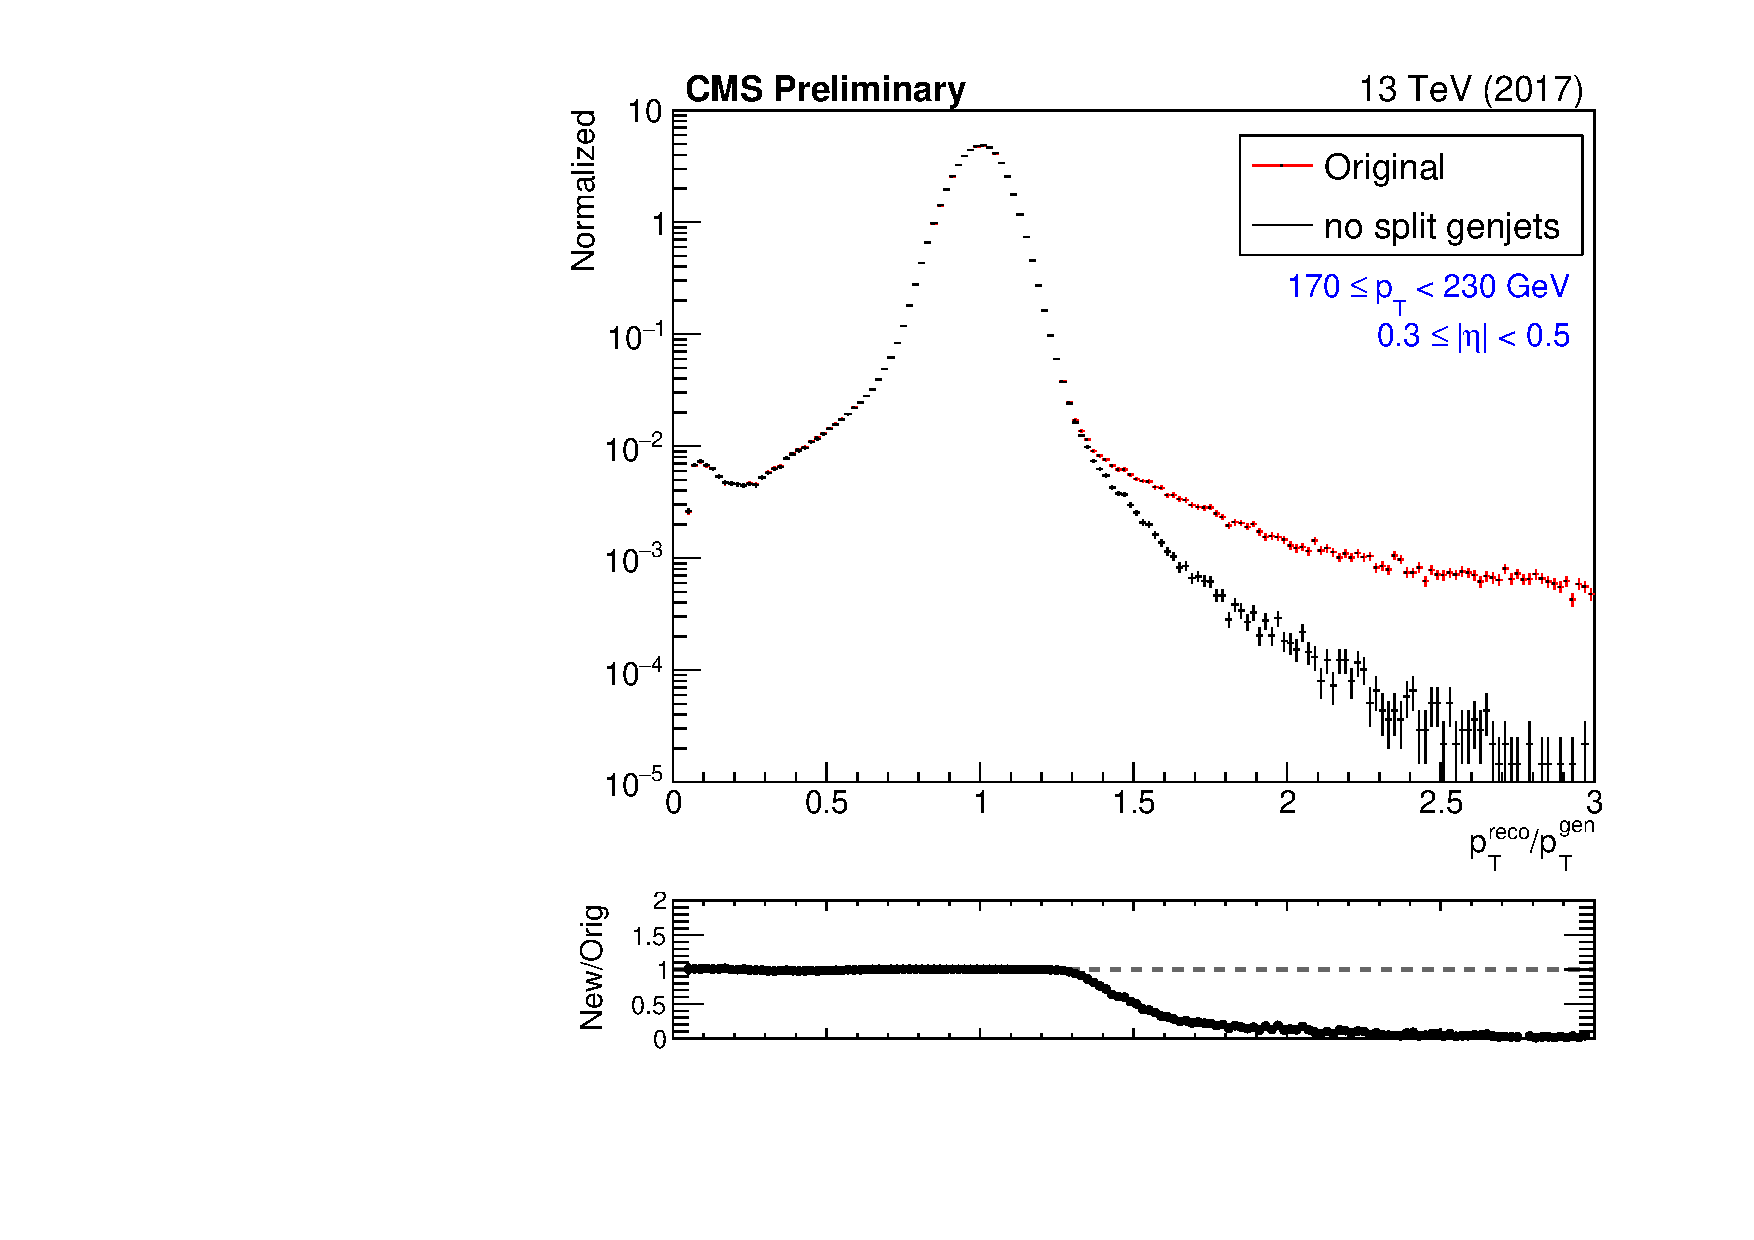
\includegraphics[width=0.325\textwidth]{figs/jetmet/compare_noSplitGen.pdf}
    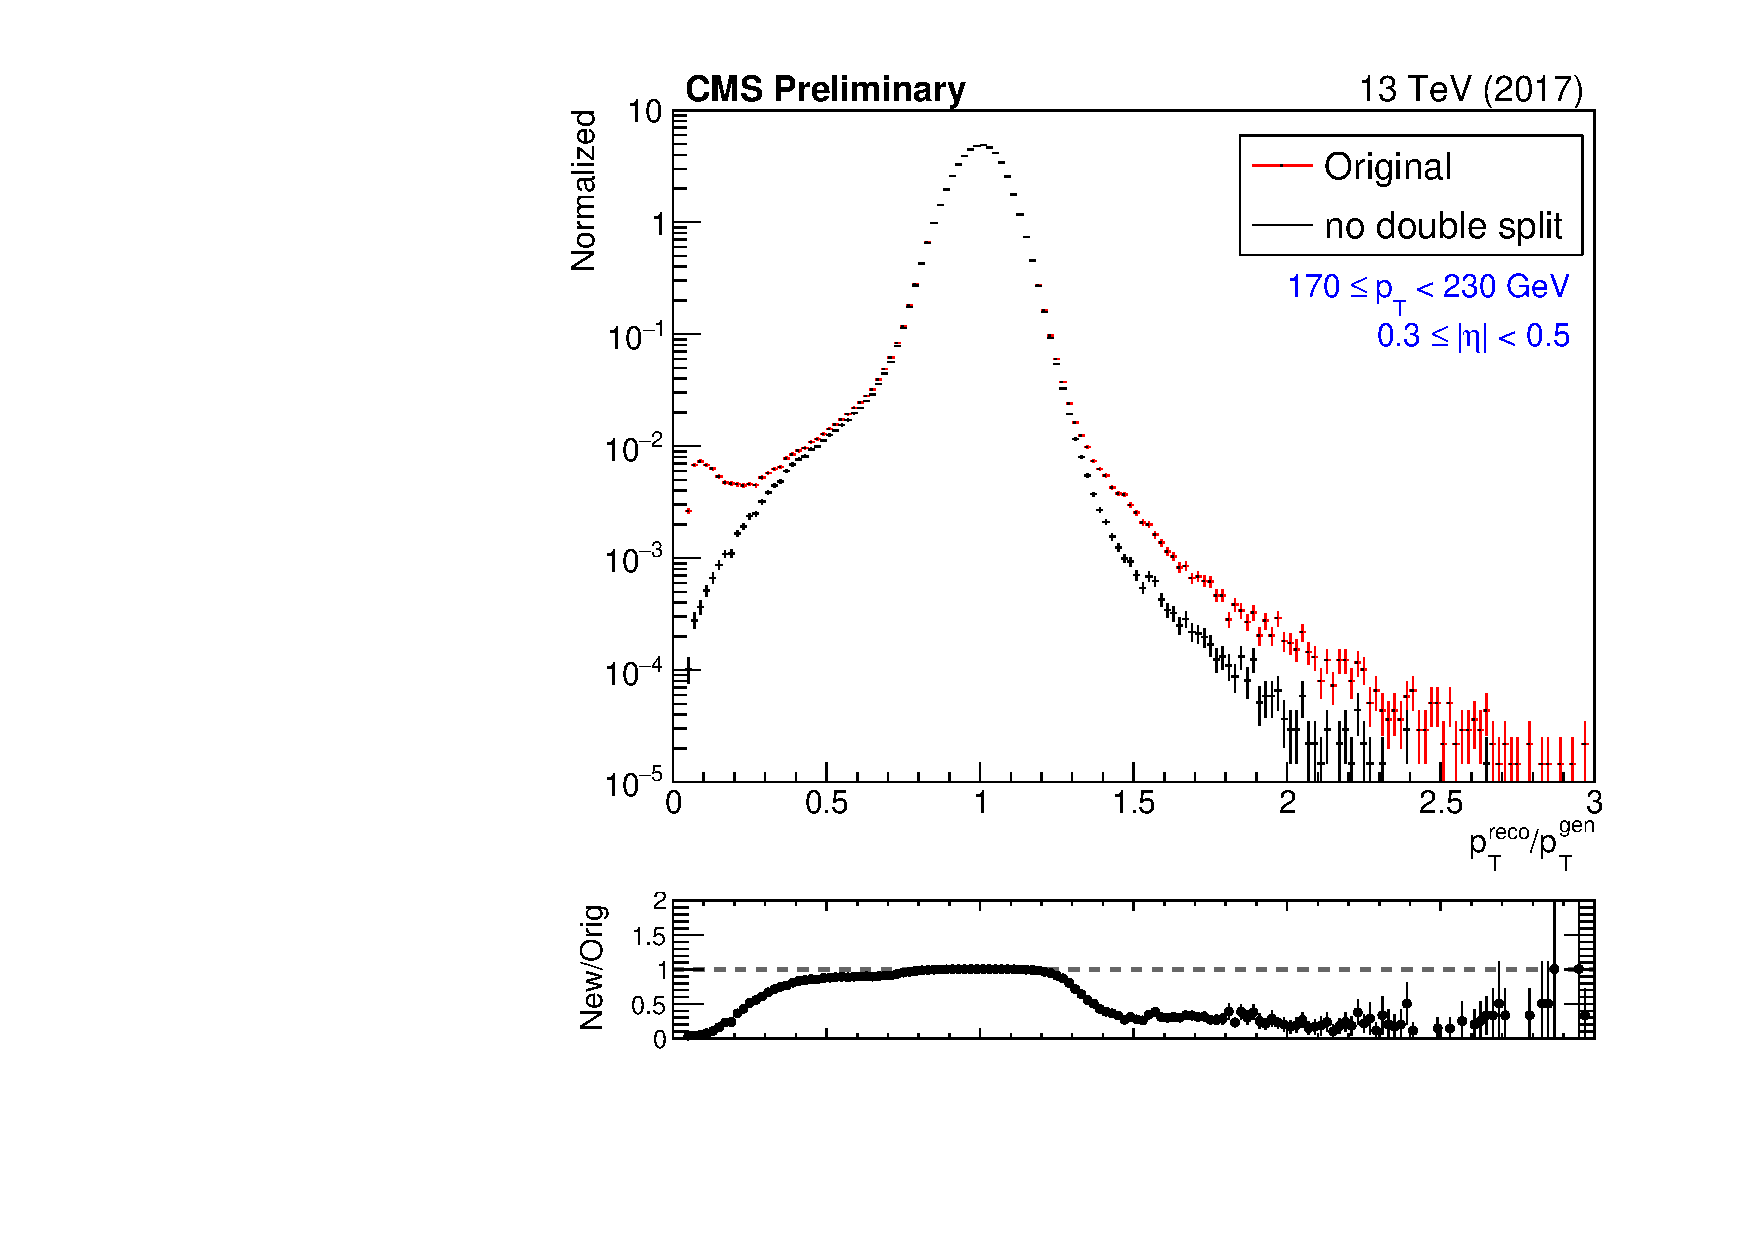
\includegraphics[width=0.325\textwidth]{figs/jetmet/compare_noDoubleSplit.pdf}
    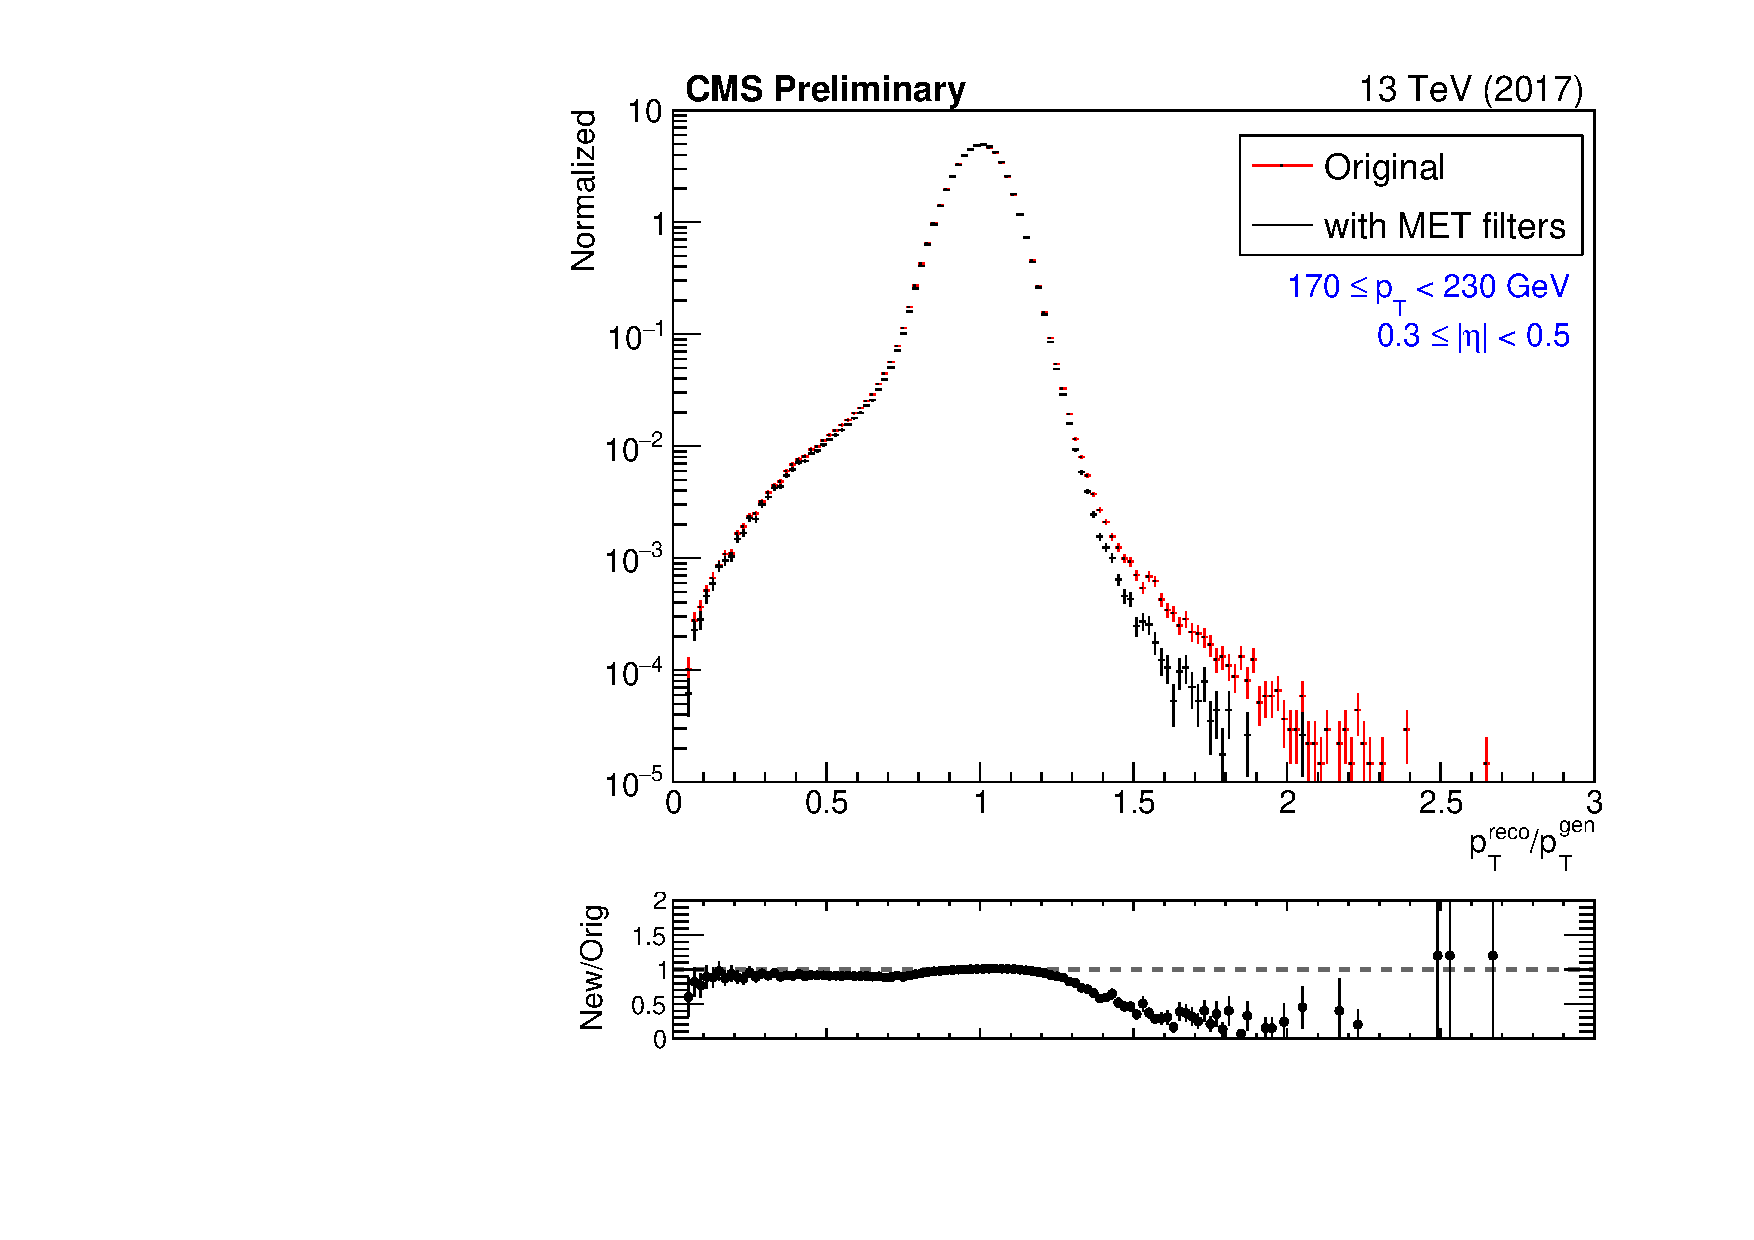
\includegraphics[width=0.325\textwidth]{figs/jetmet/compare_metFilters.pdf}
    \caption{The effect of various cuts applied during the matching on an example template (non-b jet, $170 \leq \pt < 230$\GeV, $0.3 \leq |\eta| < 0.5$).
    (left) Requiring \emph{exactly} 1 gen jet within $\text{dR}<0.3$ of a reco jet, instead of at least one. This removes ``split'' gen jets.
    (center) Requiring that there are no secondary nearby gen (reco) jets within $\text{dR}<0.5$ of the reco (gen) jet. This protects
    against splitting in both directions, so reduces both tails.
    (right) Applying MET filters and rejecting jets from events that fail. This removes bad reconstructions (e.g. fake high-\pt track) and
    primarily reduces the right tail.
    }
    \label{fig:jrt_matching_effect}
  \end{center}
\end{figure}

Step 6 throws away pairs involving a reco jet in one of a number of manually-identified ``dead'' spots in the detector.
When plotting an $\eta-\phi$ map of the jets with small ($<$0.5) $\pt^\text{reco}/\pt^\text{gen}$ values,
we observe a number of ``hot-spots'', corresponding to calorimeter regions that are dead or off in the simulation.
These do not generally correspond to real effects in the data, and lead to artificially large left tails in the templates.
We identify these regions (separately for each year) and remove any jet pairs that contain a reco jet in one of these regions.
Fig.~\ref{fig:jrt_ecalDeadCell} shows these cells highlighted for 2017 simulation on the left, and
the effect on an example template on the right.

\begin{figure}[ht]
  \begin{center}
    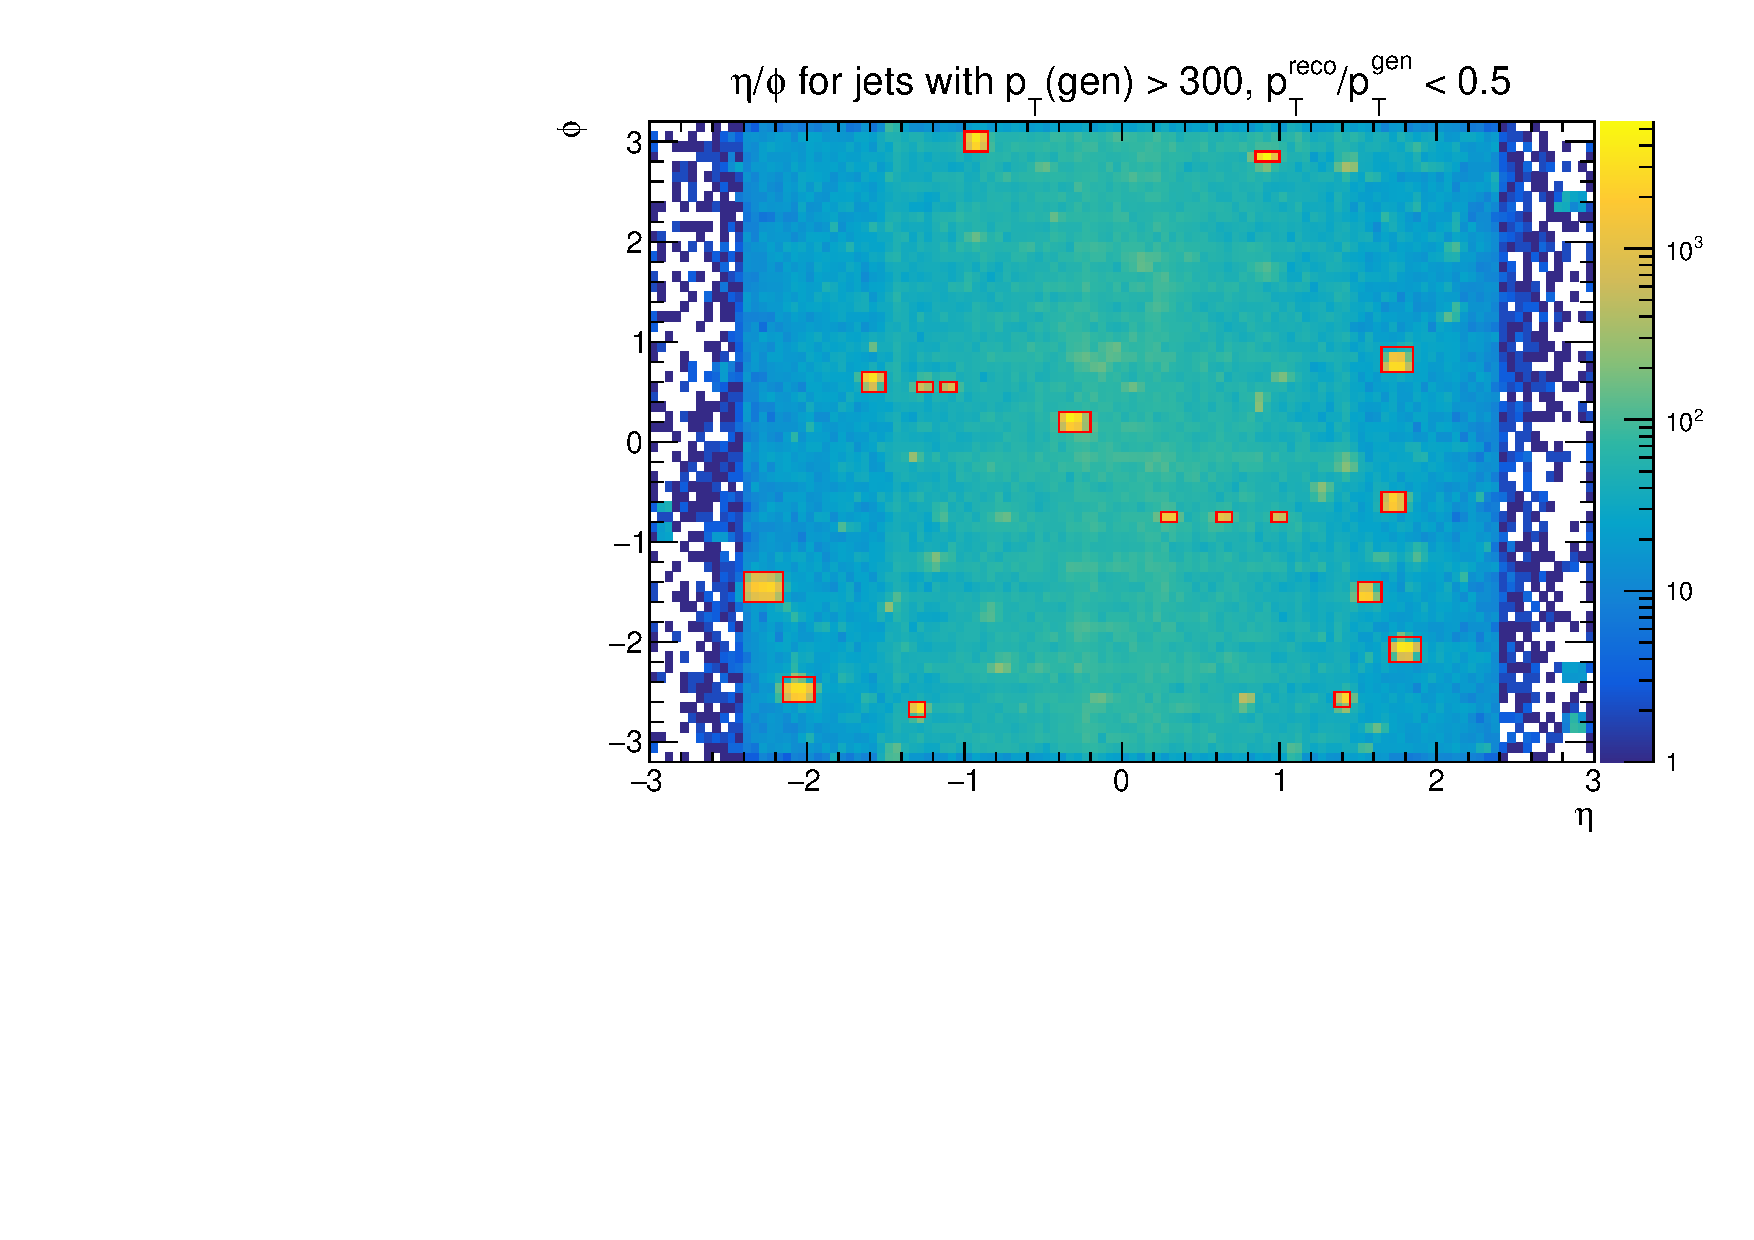
\includegraphics[width=0.54\textwidth]{figs/jetmet/ecalDeadCells.pdf}
    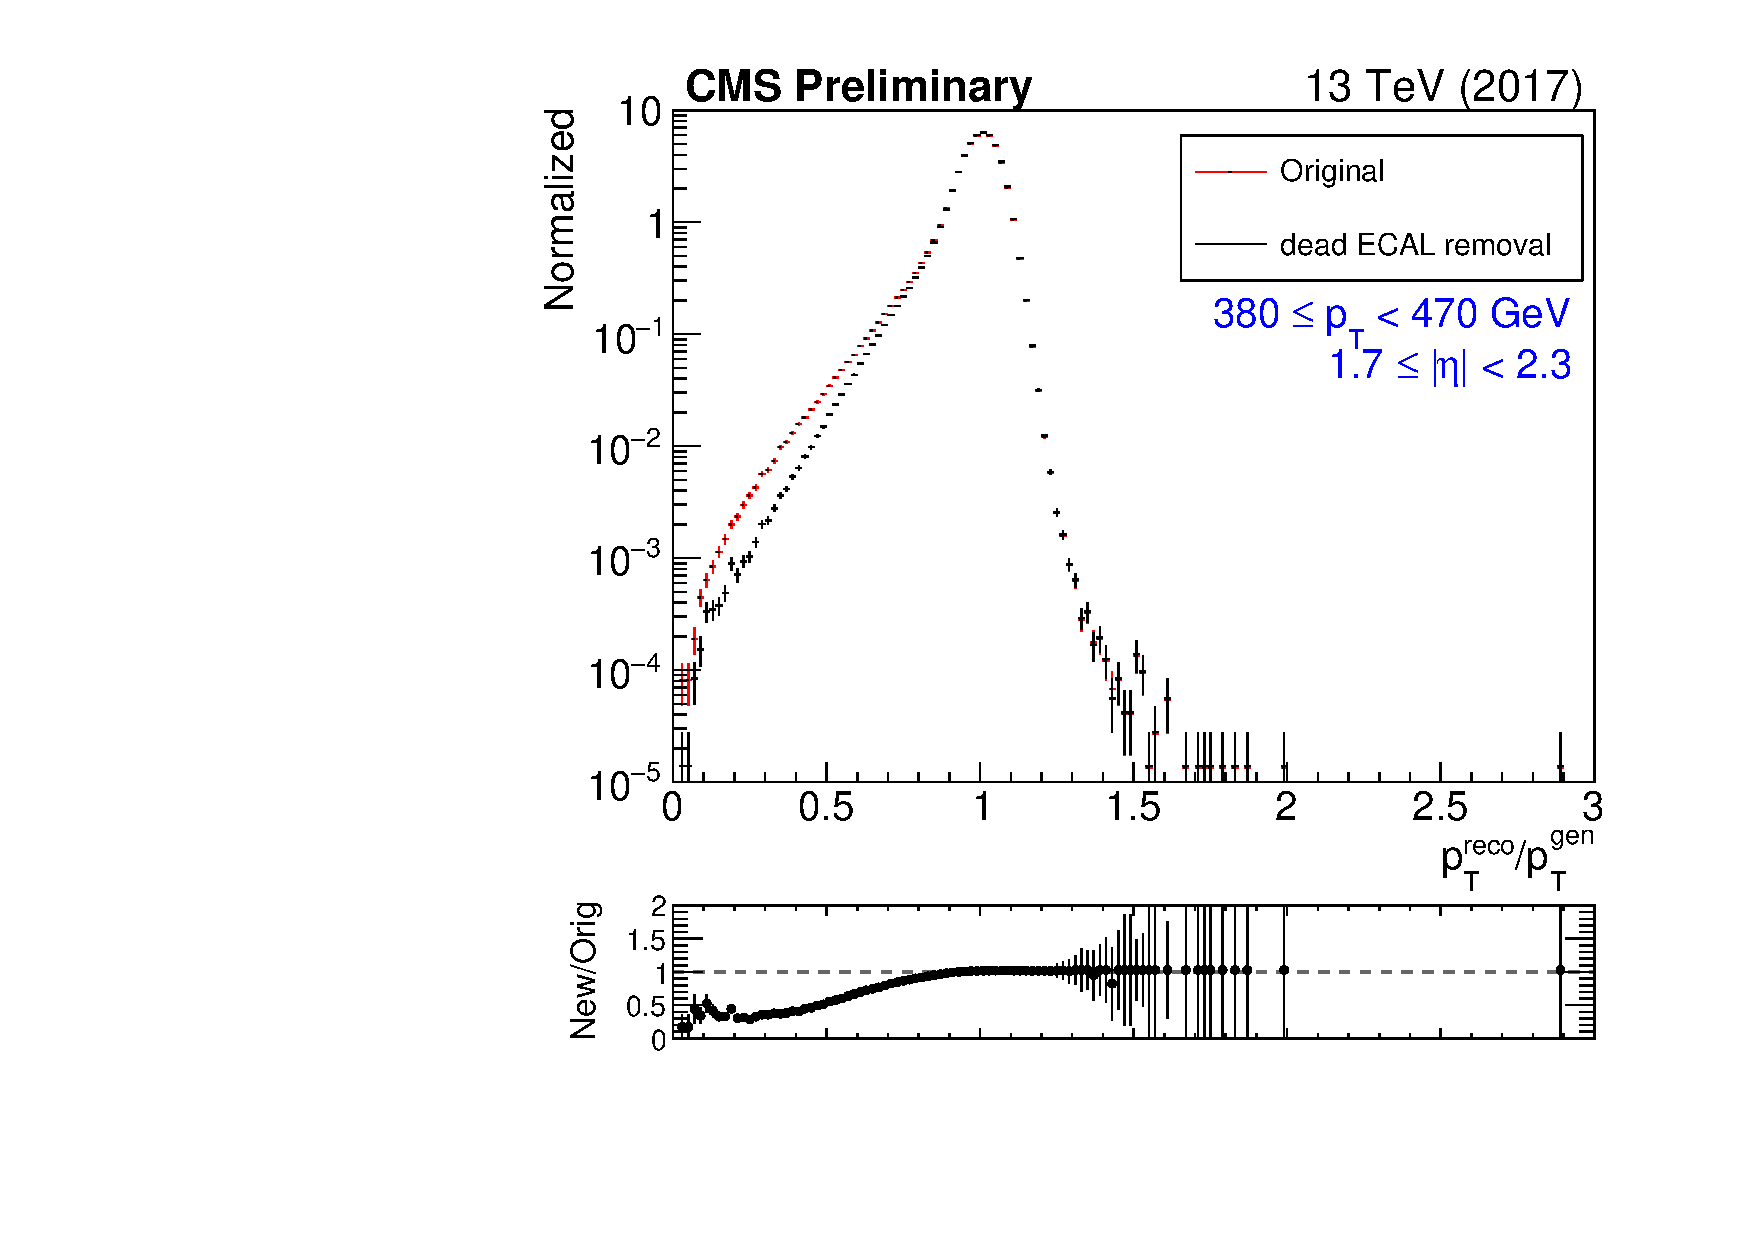
\includegraphics[width=0.45\textwidth]{figs/jetmet/compare_ecalDeadCell.pdf}
    \caption{(left) an $\eta-\phi$ map for jet pairs with $\pt^\text{gen}> 300$\GeV and
    $\pt^\text{reco}/\pt^\text{gen} < 0.5$ from 2017 simulation. Identified hot-spots
    are outlined in red. Pairs with reco jets in these regions are not used.
    (right) The effect of this removal on an example template. Relatively large reductions
    in the left tail are seen for templates containing affected regions.
    }
    \label{fig:jrt_ecalDeadCell}
  \end{center}
\end{figure}

Step 7 rejects pairs in which the reco jet fails tight jet ID.
In the main analysis, we reject the entire event if any jet with $\pt>30$\GeV
fails this ID. We apply the same ID here to avoid including these jets in 
the templates. It is found to have minimal effect, except for very high eta ($|\eta|>4.0$).

Step 8 rejects jets that fail loose pileup jet ID~\cite{JME_pileup_id}. In the rebalancing and smearing steps,
jets with $\pt<100$\GeV that fail this pileup ID are left untouched (i.e., not included
in the rebalancing and not smeared), in order to avoid trying to balance an event
against a pileup jet. Since we do not use them in the rebalancing and smearing, 
we do not want to include them in the templates.
Vetoing jets that fail pileup ID has a fairly significant effect on the tails.
At higher \pt, we see a reduction in the left tail from gen jets that were
mis-matched to a low-\pt pileup jet. At lower \pt, we see a reduction in both tails
(see Fig.~\ref{fig:jrt_jetid}).

\begin{figure}[ht]
  \begin{center}
    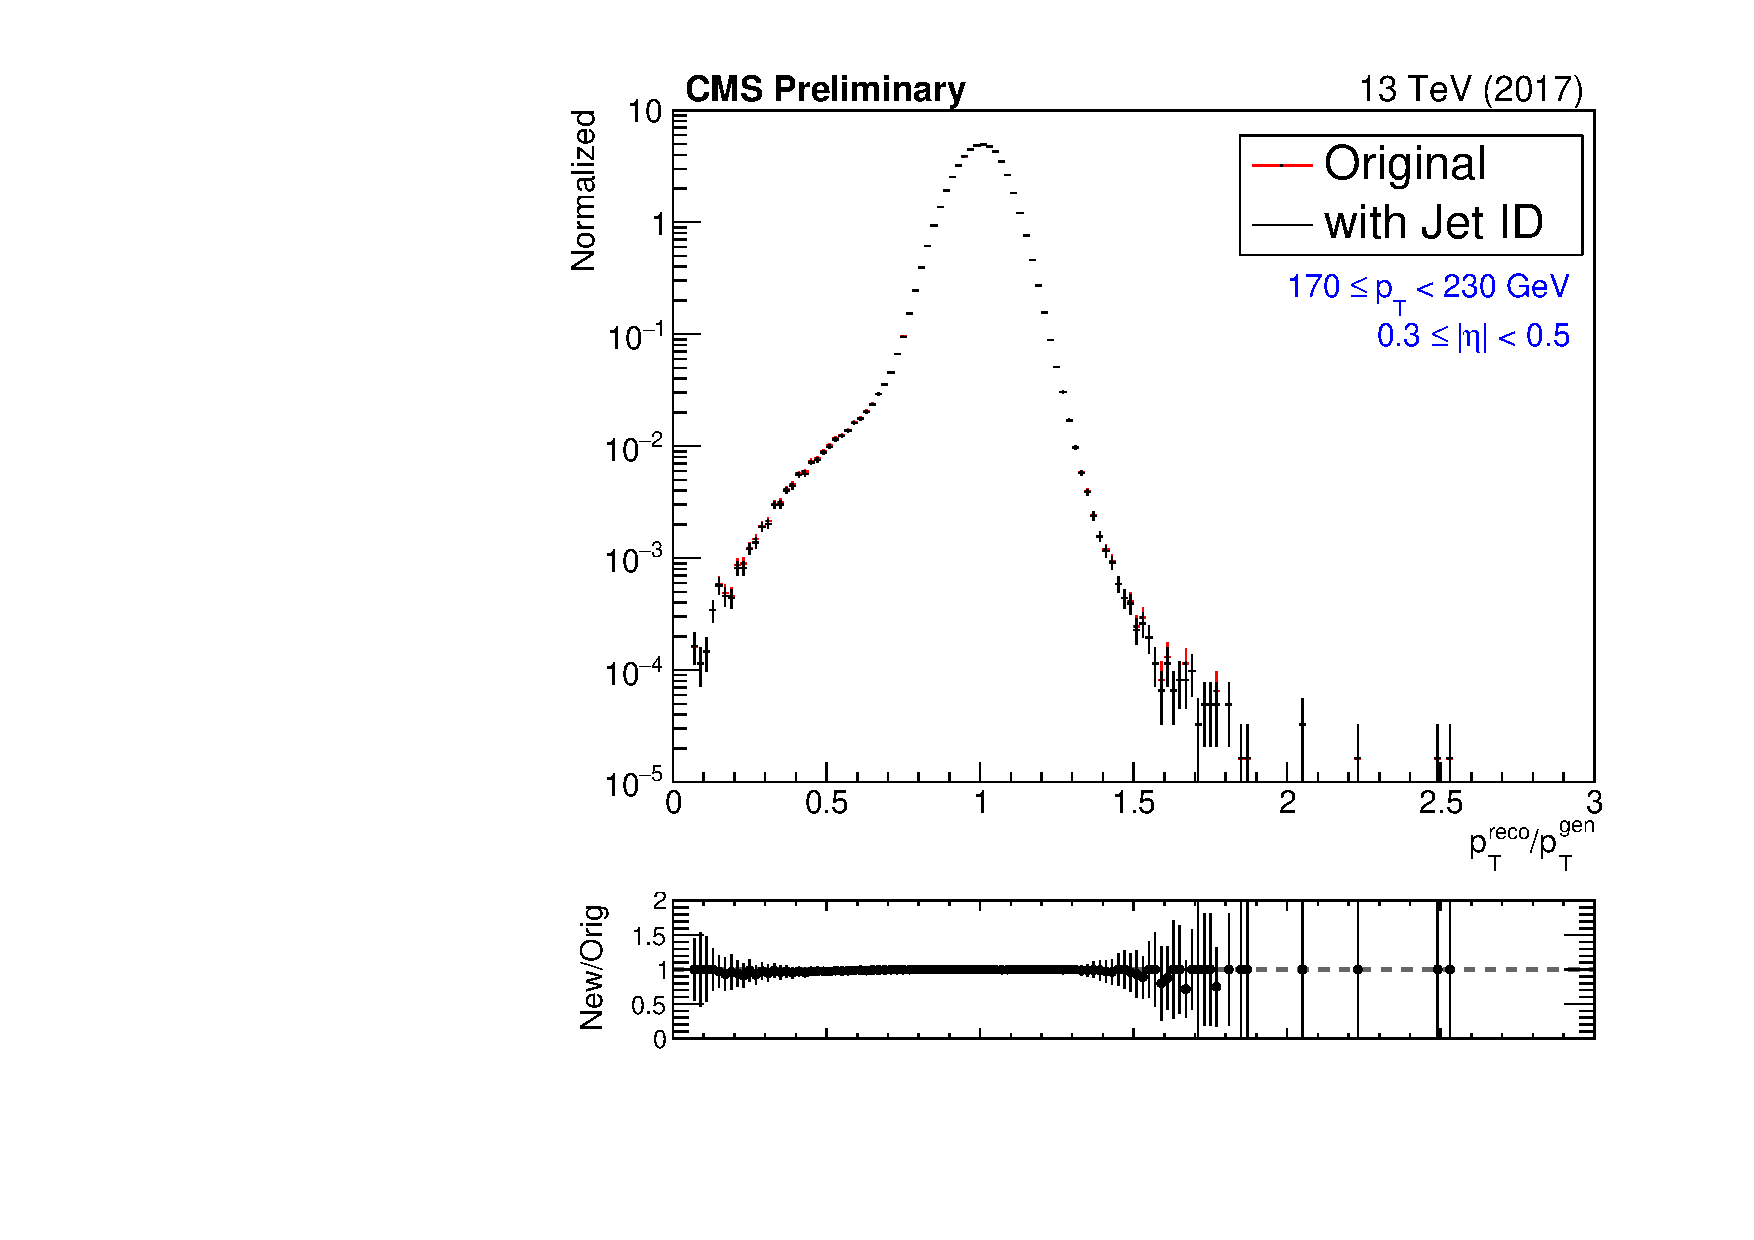
\includegraphics[width=0.325\textwidth]{figs/jetmet/compare_jetID.pdf}
    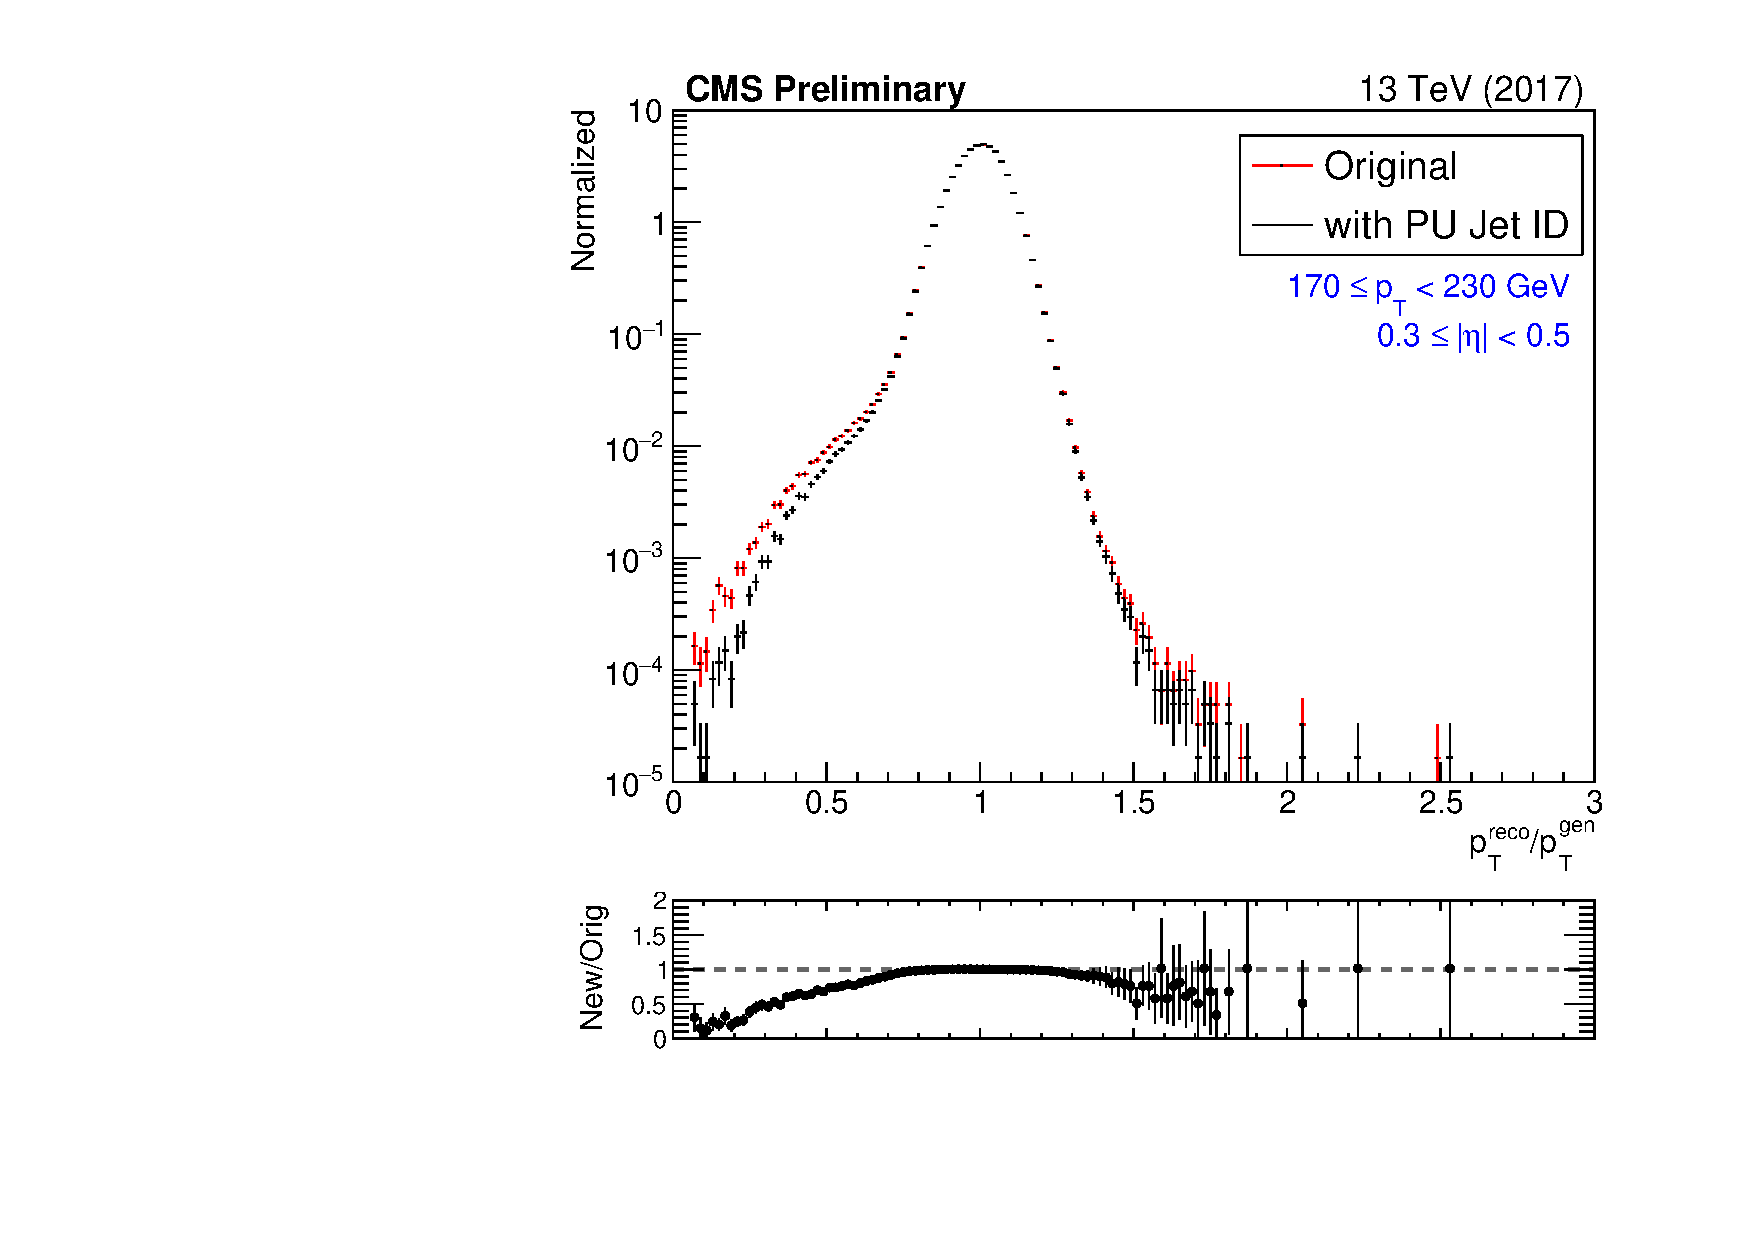
\includegraphics[width=0.325\textwidth]{figs/jetmet/compare_puJetID_highPt.pdf}
    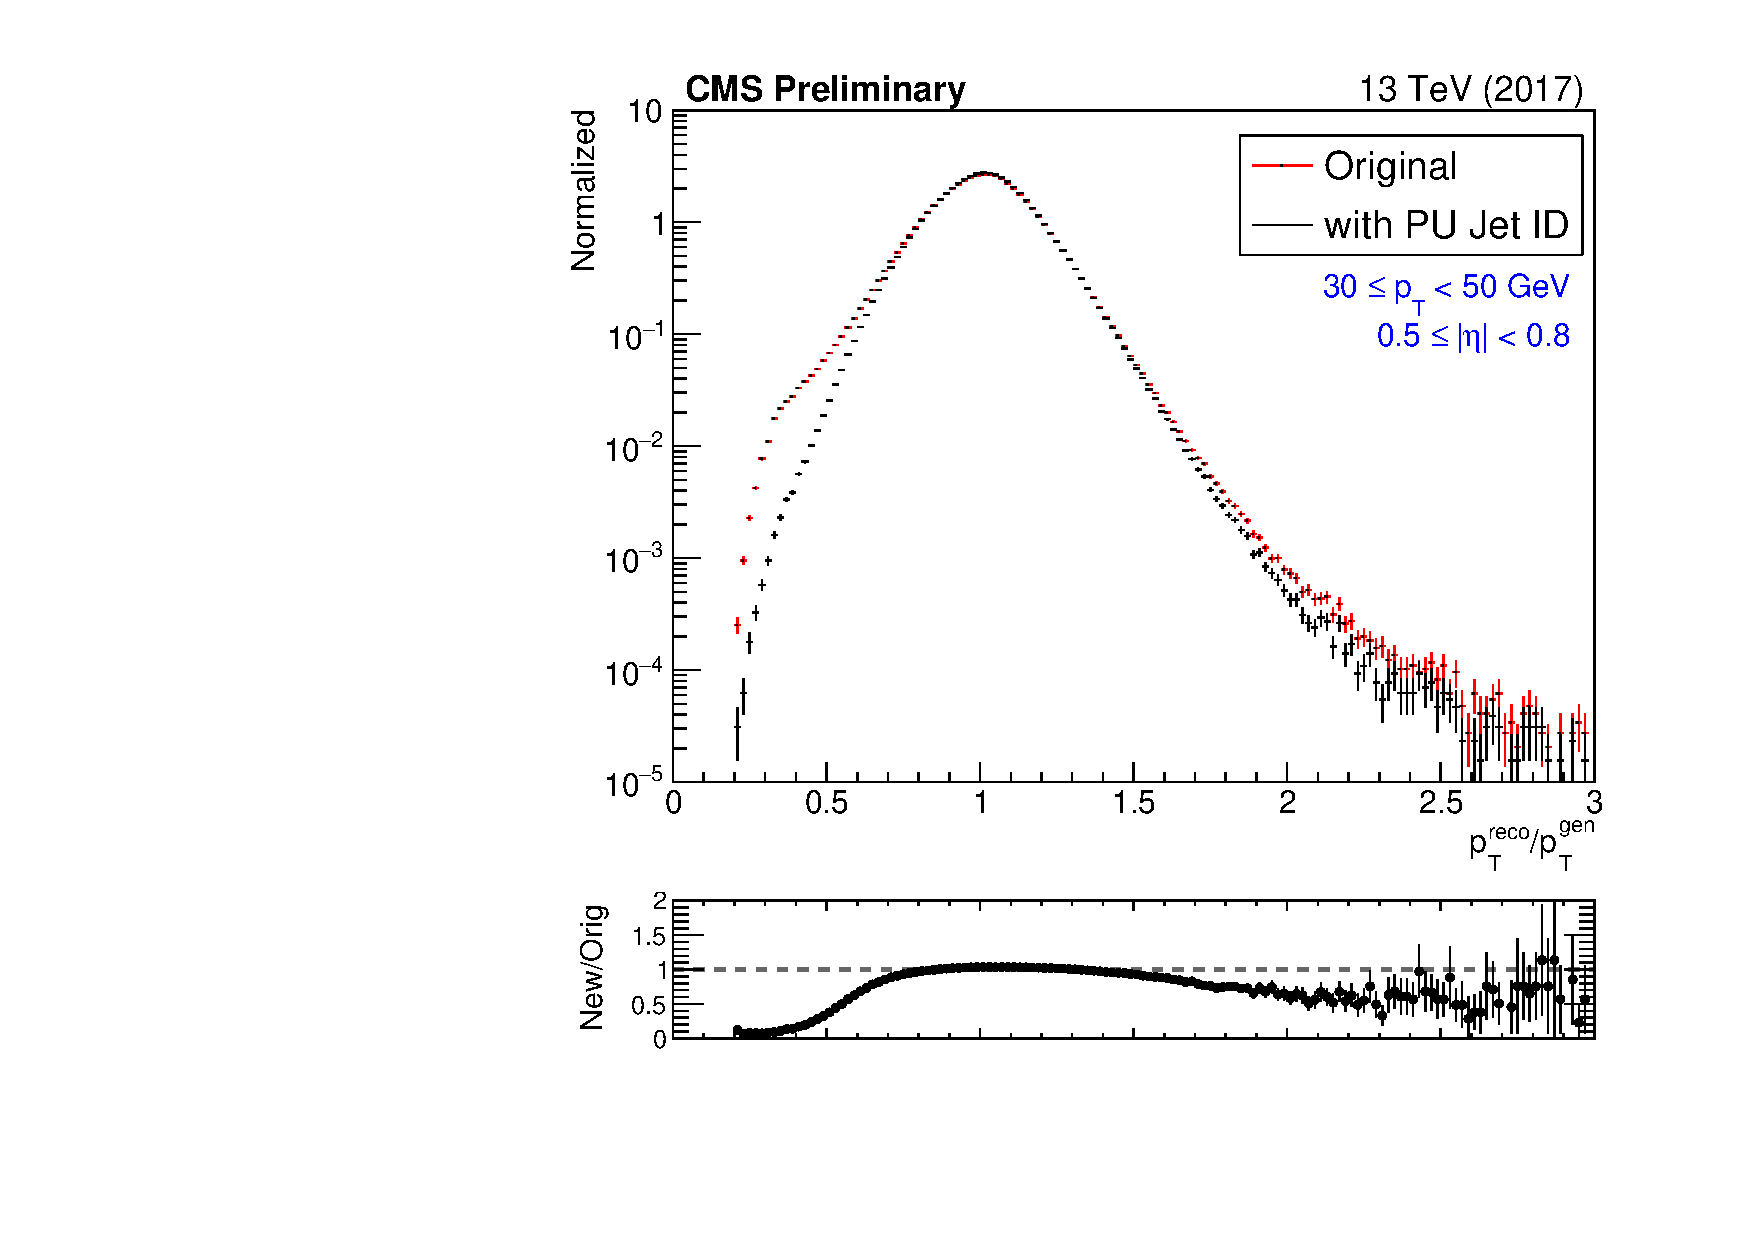
\includegraphics[width=0.325\textwidth]{figs/jetmet/compare_puJetID_lowPt.pdf}
    \caption{(left) and (center) show the effect of applying tight jet ID and loose pileup jet ID, respectively,
    to the same template as in Fig.~\ref{fig:jrt_matching_effect}. Jet ID has negligible effect,
    while the pileup jet ID leads to a reduction in the left tail.
    (right) The effect of pileup jet ID on a lower \pt template ($30\leq\pt<50$\GeV). Here we observe
    a reduction in both tails.
    }
    \label{fig:jrt_jetid}
  \end{center}
\end{figure}

In the final step, we have identified jet pairs and need to fill histograms. The only thing left to decide
is how to fill the b and non-b jet templates. There are three options that have all been tried:
\begin{enumerate}
  \item Fill only a single histogram, based on the gen jet flavor (found by identifying flavor of hadrons within jet).
  \item Fill only a single histogram, based on whether the reco jet is medium b-tagged.
  \item Fill both histograms, with weights given by the probability of tagging that jet as a b jet (corrected with data/MC scale factors).
\end{enumerate}

We evaluate each method empirically by observing the agreement in \nbtags in QCD-enriched control regions after applying
the full Rebalance and Smear method described in Chapter~\ref{chap:qcd}. It is found that (2) slightly improves on (1), and (3) is quite a bit better than both.
An example of the effect is shown in Fig.~\ref{fig:jrt_nb}.

\begin{figure}[t]
  \begin{center}
    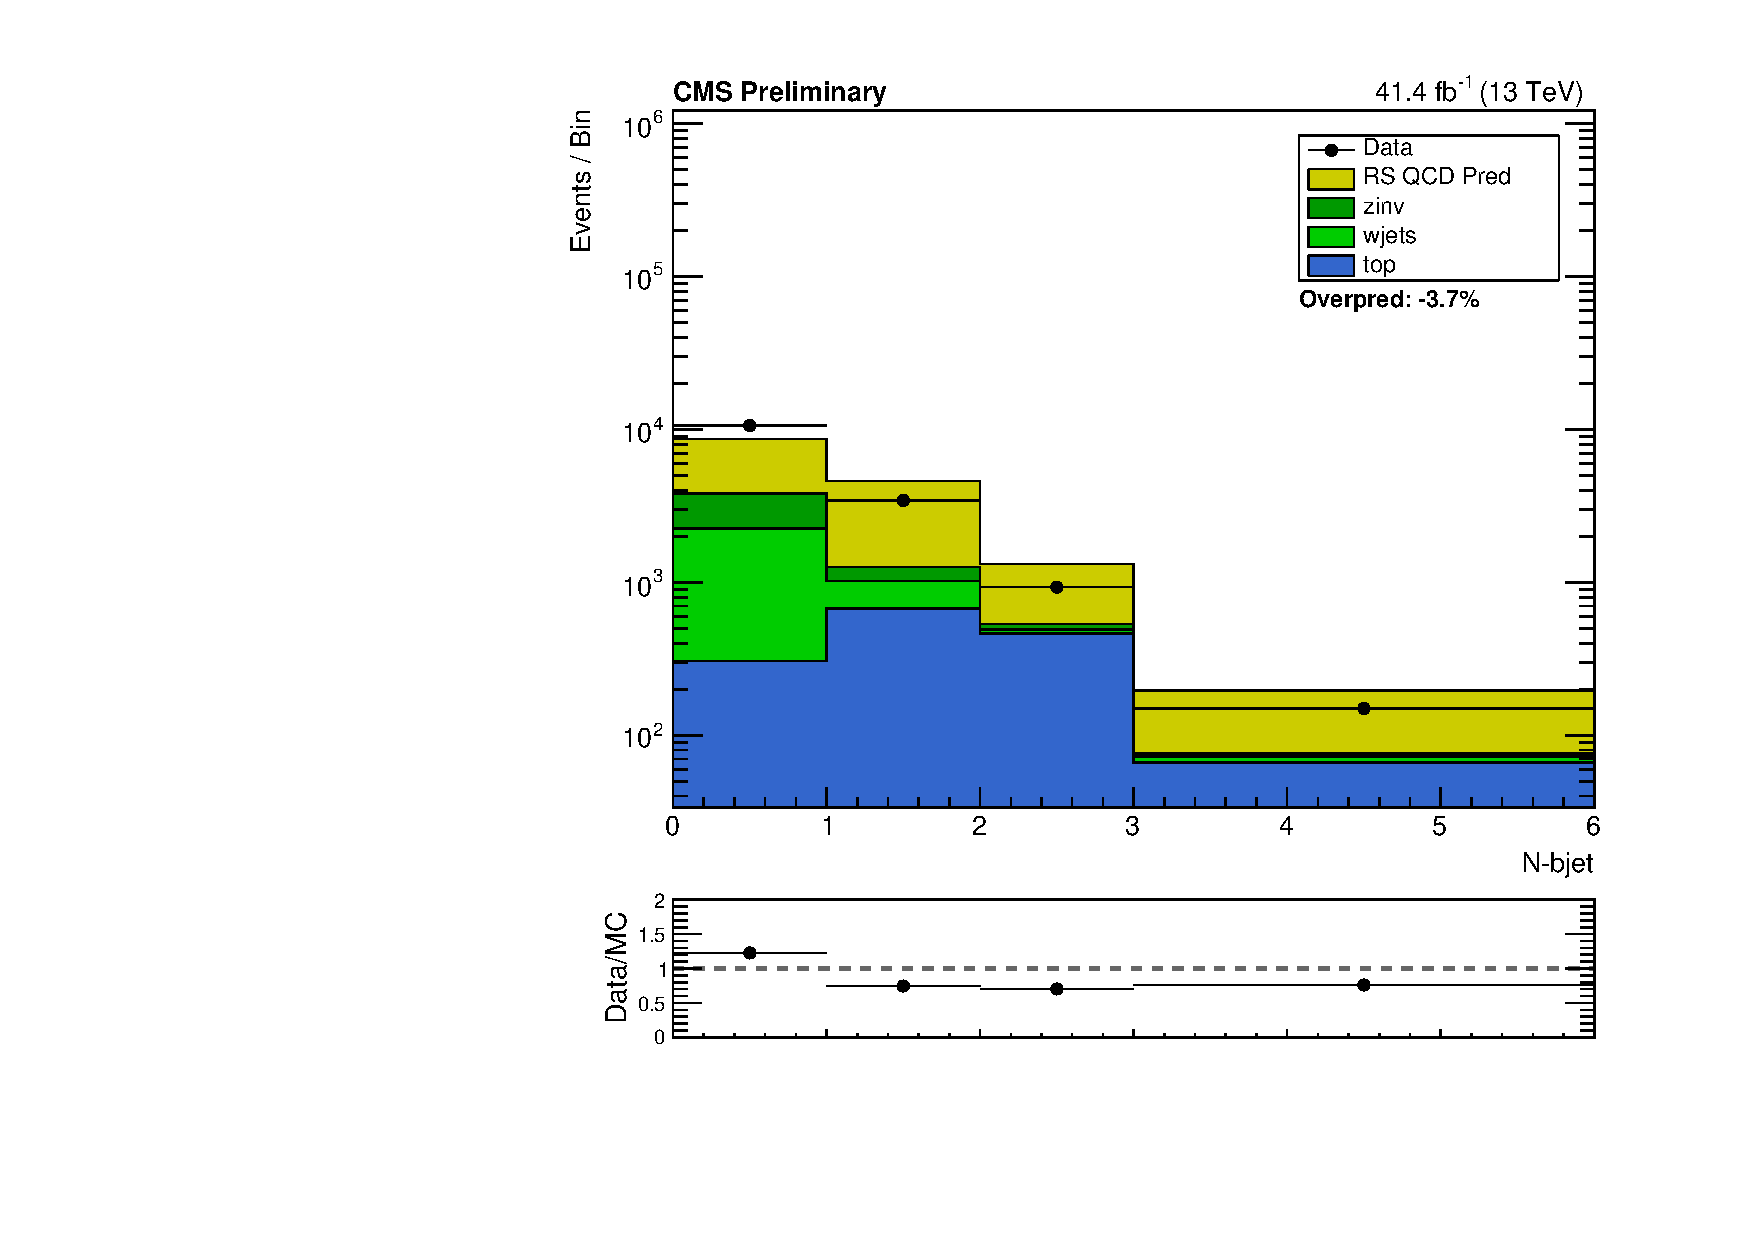
\includegraphics[width=0.49\textwidth]{figs/jetmet/nBJet20_DPhiMT2InclusiveHT450to1200_RecoBJet.pdf}
    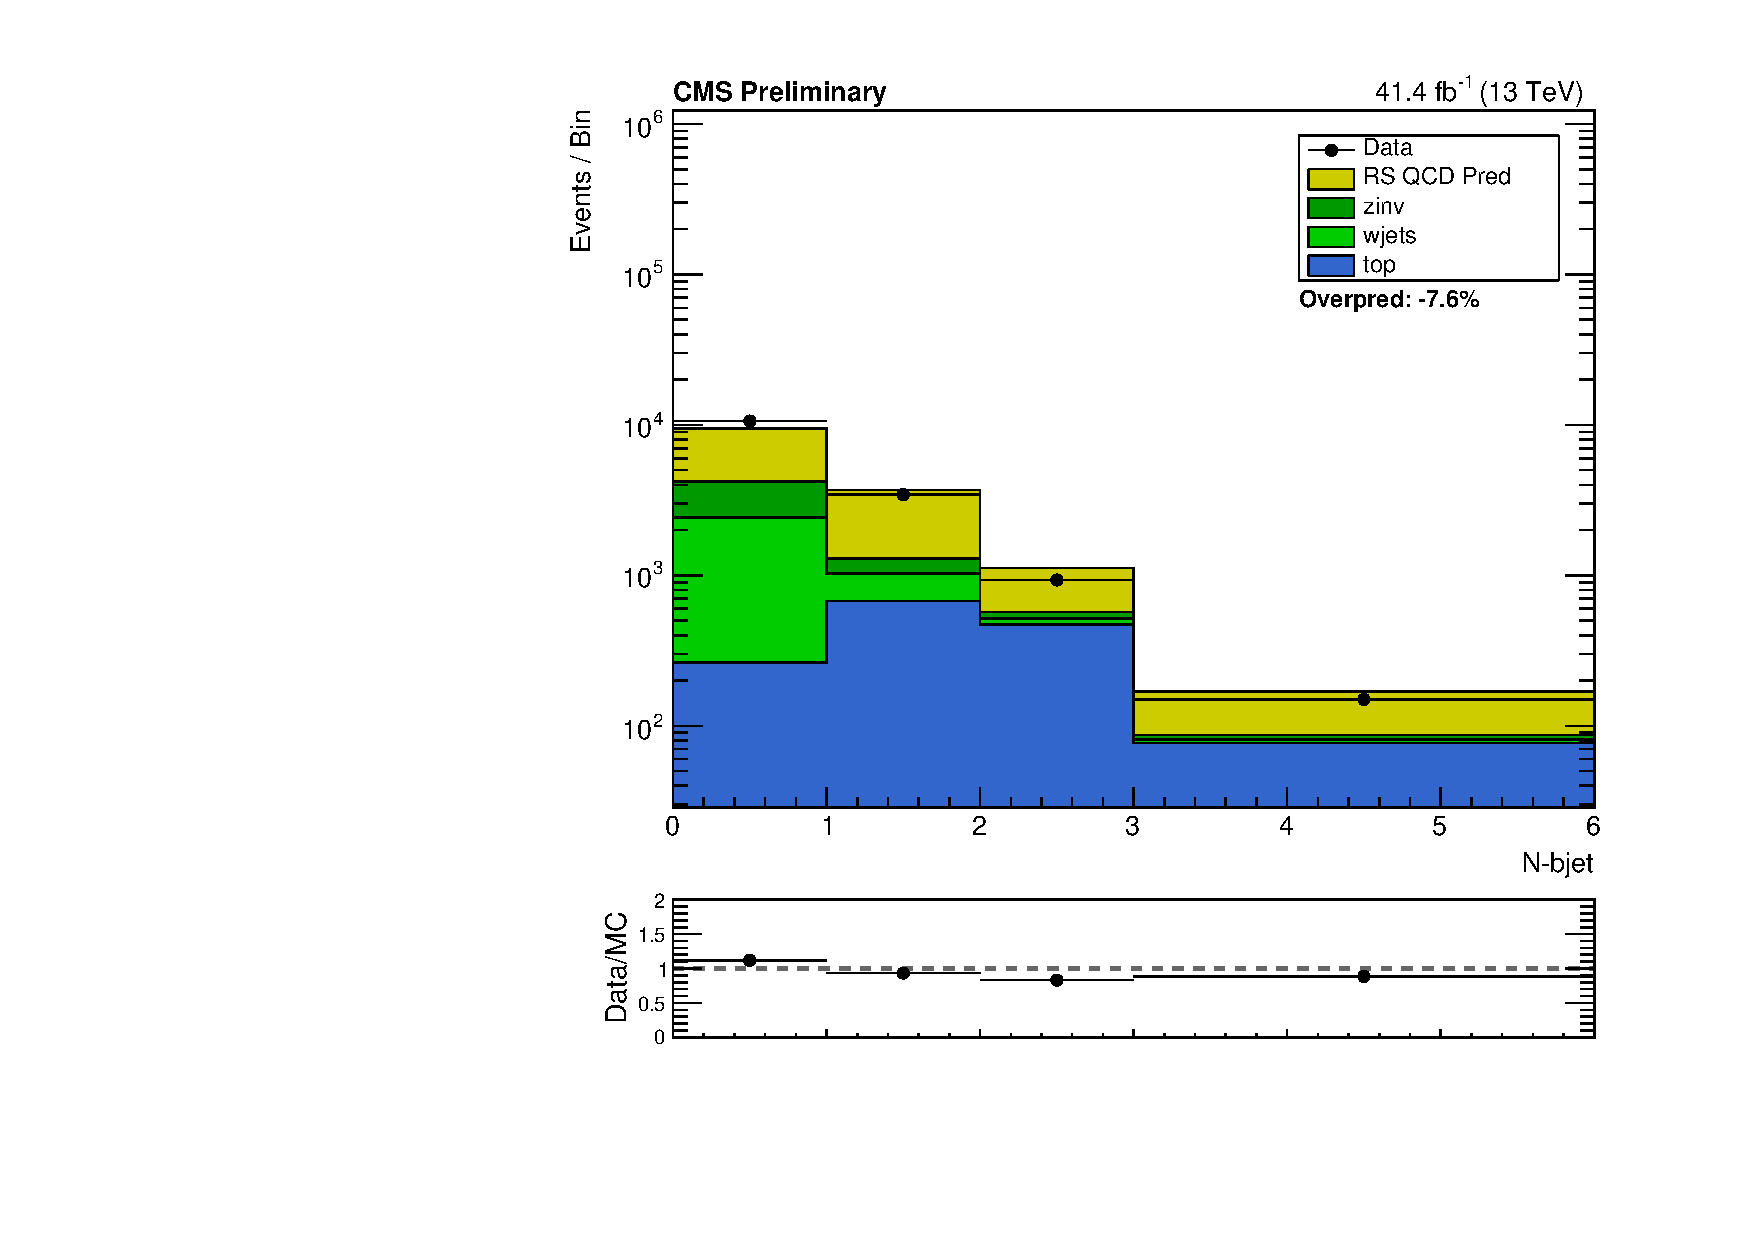
\includegraphics[width=0.49\textwidth]{figs/jetmet/nBJet20_DPhiMT2InclusiveHT450to1200_BTagSFs.pdf}
    \caption{The \nbtags distributions in the inverted-\dpmin + \mttwo sideband control region for $450 \leq \Ht < 1200$\GeV
    (described in Chapter~\ref{chap:qcd}),
    when (left) filling a single template based on reco jet medium b tagging, and (right) filling both histograms with
    weights given by the corrected probability of tagging a given jet as a medium b jet. Observed data are shown
    as black points, and prediction from the full Rebalance and Smear method is shown in yellow.
    Significant improvement is seen when using the second method. Residual shape discrepancies are 
    covered by a dedicated \nbtags shape systematic in the final estimate.
    }
    \label{fig:jrt_nb}
  \end{center}
\end{figure}


\subsection{Fits and jet energy resolution corrections}
\label{sec:jrt_fits}

Once the templates are derived, it is useful to split each template into a Gaussian ``core'' and
non-Gaussian ``tails'' The reason for this is twofold. First, it is known that jet resolution
is slightly different in data than in MC. This only applies to the standard Gaussian smearing of the jets,
so in order to correct for the differences the Gaussian core must be isolated.
Second, is is useful for studies on systematics to be able to alter the core/tails of the
templates individually. For example, to study the effect of mis-modeling in the tails,
one should be able to modify the size of the tails without affecting the size/shape
of the Gaussian core.

To fit the core of a template, a Gaussian is fitted in the range (mean $\pm$ RMS), where mean and RMS
are the mean and standard deviation of the template.
When measuring jet energy resolution and deriving scale factors, CMS only defines the core
of the jet response function as extending out to $\pm2\sigma$ of the fitted Gaussian~\cite{JME_jes_jer}.
To be consistent, we use the same definition here, and in order to avoid discontinuities,
we linearly scale the Gaussian to 0 between $\pm1$ and 2 $\sigma$. More precisely, if $g(x)$ is the
full fitted Gaussian, and $\mu$ and $\sigma$ are its mean and standard deviation, our defined core function is
\[
\text{Core}(x) = 
\begin{cases}
g(x) & \text{if } |x-\mu| \leq 1\sigma \\
g(x)\left(2-\frac{|x-\mu|}{\sigma}\right) & \text{if } 1\sigma < |x-\mu| \leq 2\sigma \\
0 & \text{if } |x-\mu| > 2\sigma \\
\end{cases}.
\]

The tails are then simply defined as the full template function minus $\text{Core}(x)$.
Examples of this fitting procedure are shown in Fig.~\ref{fig:jrt_examples}. The truncated-Gaussian
cores are shown in red, and the tails in green.

The first way that these fits are used is in the correction of the templates for jet energy resolution
differences between data and MC. The JetMET group provides year-dependent scale factors binned in 
$\eta$, shown in Table~\ref{tab:jrt_jersfs}. When smearing data events, the core of the template for a given jet
is widened by this scale factor before drawing a random smear factor from the distribution. This is done in a 
way to preserve the relative core/tail normalization. Specifically, if $\alpha$ is the scale factor by which we
want to widen the core, the modified template is given by
\[
f_\alpha(x) = \frac{1}{\alpha}\cdot\text{Core}((x-1)/\alpha+1) + \text{Tail}(x).
\]

\begin{table}[t]
\caption{Jet energy resolution scale factors (data resolution divided by MC resolution) provided by the JetMET group.
             Uncertainties are statistical plus systematic.}
\label{tab:jrt_jersfs}
\centering
%\small
\begin{tabular}{|c|ccc|}
\hline
 & 2016 & 2017 & 2018 \\ \hline
$0.0 \leq |\eta| < 0.5$ & $1.160\pm0.065$ & $1.143\pm0.022$ & $1.150\pm0.042$ \\
$0.5 \leq |\eta| < 0.8$ & $1.195\pm0.065$ & $1.182\pm0.048$ & $1.134\pm0.080$ \\
$0.8 \leq |\eta| < 1.1$ & $1.146\pm0.063$ & $1.099\pm0.046$ & $1.102\pm0.052$ \\
$1.1 \leq |\eta| < 1.3$ & $1.161\pm0.103$ & $1.114\pm0.140$ & $1.134\pm0.112$ \\
$1.3 \leq |\eta| < 1.7$ & $1.128\pm0.099$ & $1.131\pm0.147$ & $1.104\pm0.211$ \\
$1.7 \leq |\eta| < 1.9$ & $1.100\pm0.108$ & $1.160\pm0.097$ & $1.149\pm0.159$ \\
$1.9 \leq |\eta| < 2.1$ & $1.143\pm0.121$ & $1.239\pm0.191$ & $1.148\pm0.209$ \\
$2.1 \leq |\eta| < 2.3$ & $1.151\pm0.114$ & $1.260\pm0.150$ & $1.114\pm0.191$ \\
$2.3 \leq |\eta| < 2.5$ & $1.296\pm0.237$ & $1.409\pm0.202$ & $1.347\pm0.274$ \\
$2.5 \leq |\eta| < 2.8$ & $1.342\pm0.209$ & $1.991\pm0.568$ & $2.137\pm0.524$ \\
$2.8 \leq |\eta| < 3.0$ & $1.779\pm0.201$ & $2.292\pm0.374$ & $1.650\pm0.941$ \\
$3.0 \leq |\eta| < 3.2$ & $1.187\pm0.124$ & $1.270\pm0.109$ & $1.225\pm0.194$ \\
$|\eta| \geq 3.2$       & $1.192\pm0.149$ & $1.154\pm0.152$ & $1.082\pm0.198$ \\
\hline
\end{tabular}
\end{table}

To assign a systematic from uncertainty in the jet energy resolution modeling, the smearing is run three times:
once using the central values in Table~\ref{tab:jrt_jersfs}, once with the $+1\sigma$ values,
and once with the $-1\sigma$ values. The differences in final signal region predictions,
integrated over each \Ht region, are used to assign a systematic uncertainty. The results of this
procedure are shown in Fig.~\ref{Fig:rs_data_JER_var} in Sec.~\ref{sec:rs_jrt_core}.

The fitted tails are used in a similar way to assign a systematic due to uncertainty in the tail modeling.
The tails are not stretched along the $x$ direction, but instead simply scaled up/down (i.e., their normalization
relative to the core is increased/decreased). Formally, to increase the tail size by a factor $\beta$, the
modified template is given by
\[
   f_\beta(x) = N_\beta(\text{Core}(x) + \beta\cdot\text{Tail}(x)),
\]
where $N_\beta$ is a normalization factor to ensure that the template integral remains equal to one.
Results of applying this procedure to the smearing of QCD MC with $\beta=1.25$ and 1.50 
are shown in Fig.~\ref{Fig:rs_modify_tail} in Sec.~\ref{sec:rs_jrt_tail}. 
The differences in final signal region yields with $\beta=1.25$ are used to assign a systematic uncertainty.
